\section{Faithful Generation}
\label{sec:nlgfg}


Let $\GEN : \mrspace \rightarrow \outSpace$ be an arbitrary mapping from 
\meaningrepresentation~to utterance. We say that a mapping $\GEN$ is 
\faithful~if we have that \[\denotes{\GEN(\mr)} = \mr \quad \forall \mr: \mr \in \mrspace.\] In words,
$\GEN$ is faithful if the propositional content of $\mr$ (i.e., the semantics
of the \attributevalue~pairs in $\mr$) is correctly expressed by the 
generated utterance $\predutttoks = \GEN(\mr)$ for any wellformed \meaningrepresentation~$\mr$. 

If $\GEN$ is implemented with a template-style method like in \citet{e2etmepl},
it is possible to design a faithful mapping. However, it is possible that 
faithfuless and naturalness are in tension, as the method of \citet{e2etempl}
did not performance highly on human judgements of naturalness.

It is well known that implementing $\GEN$ with a neural mode $\gen$ and 
an inference procedure like beam search are not sufficient to obtain a faithful
model.  The bias inherent to beam search means that 
low-perplexity utterances are 
more likely to be generated \cite{beamsucks}. 
 A common approach to make $\gen$ more faithful is to perform overgeneration 
 with
reranking. 
The $\nbest$-best list of utterances $\nbestlist = \left\{\utttoks^{(1)},\ldots,
\utttoks^{(\nbest)}\right\}$ is produced using beam search on $\gen\left(\cdot|\ls(\mr);\params \right).$
Then 
a descriminiative model $\dmodel$ is used to rerank $\nbestlist$ such
that the final return utterance is \[
\predutttoks = \argmax_{\utttoks \in \nbestlist} \dmodel\left(\mr\vert\utttoks;\dparams\right). \]
In this setting, $\dmodel$ can be understood as a 
\meaningrepresentation~parser, and the new inference procedure selects the 
utterance that 
that most likey denotes the input $\mr$ under $\dmodel$. While this reduces the risk of
generating an incorrect utterance with respect to $\mr$, it can still fail
when either $\dmodel$ is not accurate or when $\nbestlist$ does not contain
a completely correct utterance.

This is compounded by the finding that neural models on natural language data\footnote{Here we are referring to both \sequencetosequence~models but also 
sequence classification and sequence-pair classification }  do not 
naively exhibit the quality of systematicity \citep{fodor,genwosys}, or 
the ability to exploit the algebraic and compositional 
nature of natural language. \citet{genwosys} give the example of a human
speaker that understands the concept of ``twice'' or ``again,'' who, upon
learning a novel verb, ``to dax,'' immediately understands the meaning 
of ``daxed twice'' or ''to dax again'' even though they have never seen 
examples of these compositions before. Empirically, they demonstrate that a
\recurrentneuralnetwork~based \meaningrepresentation-to-text model ({\color{red} check direction}) does not posses this ability and frequently fails to 
generalize to novel compostions even where the individual constituents of 
the compositinoal phrases are well represented in the training distribution.

In our present case, this failure of systematicy manifests itself a failure
to realize individual \attributevalues~that are well represented in the 
training data when those \attributevalues~occur in novel \meaningrepresentations at test time. We use as a case-study, the \attributevalue~``near=Burger King.'' which in our restaurant domain data, denotes that a restaurant $x$ is near
Burger King. (TODO mention dataset).

The \attributevalue~\AV{near}{Burger King} appears frequently in the training
data in longer \meaningrepresentation/utterance pairs. In fact \AV{near}{Burger King} is positively associated with \meaningrepresentations where seven or eight \attributes~are specified (there are eight total unique attributes on this
dataset). See \autoref{bkpmi} where we plot the point-wise mutual information
(PMI) \citep{chruch1990} of the occurrence of the \AV{near}{Burger King} and the occurrence of a \meaningrepresentation~of a particular size\footnote{The size of a \meaningrepresentation~$\setsize{\mr}$ is the number of \attributevalue~pairs in $\mr$.} on the training set, where the PMI is computed as 
\[\pmi(\AV{near}{Burger King},  \setsize{\mr} = k) = \log \frac{p(\AV{near}{Burger King}, \setsize{\mr} = k)}{p( \AV{near}{Burger King}  ) p(\setsize{\mr} = k)}     \quad \forall k : k \in \{3,\ldots,8\},\]
with \begin{align*}
    p(\AV{near}{Burger King}) &= \frac{\sum_{(\mr,\utttoks) \in \corpus}\mathds{1}\left\{ \AV{near}{Burger King} \in \mr \right\}}{\setsize{\corpus}} \\
    p(\setsize{\mr}=k) &= \frac{\sum_{(\mr,\utttoks) \in \corpus}\mathds{1}\left\{ \setsize{\mr} = k \right\}}{\setsize{\corpus}} \\
    p(\AV{near}{Burger King},\setsize{\mr}=k) &= \frac{\sum_{(\mr,\utttoks) \in \corpus}\mathds{1}\left\{\AV{near}{Burger King} \in \mr \wedge \setsize{\mr} = k \right\}}{\setsize{\corpus}}.
\end{align*}


We trained a uni-directional GRU variant of $\gen$ on the training corpus
$\corpus$ and then tried to generate an utterance for the following \meaningrepresentation,
\begin{center}
    \MR{\textsc{Inform}}
        {\AV{name}{Alimentum}}  
        {\AV{near}{Burger King}}
        {\AV{area}{city centre}}
        {\AV{family\_friendly}{no}}\end{center}
using beam search. Notice that in this case $\setsize{\mr}=4$ in this case,
indicating that the occurrence of \AV{near}{Burger King} is novel given
 the training set.
We see some beam search canditates below, {\color{red}\uline{underlining in red}} the phrases that
are not semantically correct given the \meaningrepresentation,

\begin{enumerate}
\item Alimentum is located in the city centre {\color{red}\uline{near the Express by Holiday Inn.}} It is not family-friendly.     
\item Alimentum is located in the city centre {\color{red}\uline{near the Yippee Noodle Bar.}} It is not family-friendly.
\item Alimentum is located in the city centre {\color{red}\uline{near the Raja Indian Cuisine.}} It is not family-friendly.
\item Alimentum is not family-friendly. It is located in the city centre {\color{red}\uline{near the Yippee Noodle Bar.}}
\item The Alimentum is located in the city centre {\color{red}\uline{near the Express by Holiday Inn.}} It is not family-friendly.
%Alimentum is not family-friendly. It is located in the city centre near the Raja Indian Cuisine.\\\vspace{-1em}\\
%Alimentum is located in the city centre near the Clare Hall. It is not family-friendly.\\\vspace{-1em}\\
%Alimentum is located in the city centre near the crowne plaza hotel. It is not family-friendly.\\\vspace{-1em}\\
%Alimentum is not family-friendly. It is located in the city centre near the express by holiday inn.\\\vspace{-1em}\\
%The Alimentum is located in the city centre near the Yippee Noodle Bar. It is not family-friendly.\\\vspace{-1em}\\
%Alimentum is not family-friendly. It is located in the city centre near the Clare Hall.\\\vspace{-1em}\\
%The Alimentum is located in the city centre near the Raja Indian Cuisine. It is not family-friendly.\\\vspace{-1em}\\
%In the city centre near the express by holiday inn is Alimentum. It is not family-friendly.\\\vspace{-1em}\\
%Alimentum is located in the city centre near the city centre. It is not family-friendly.\\\vspace{-1em}\\
%Alimentum is located in the city centre near the rice boat. It is not family-friendly.\\\vspace{-1em}\\
%The Alimentum is not family-friendly. It is located in the city centre near the Yippee Noodle Bar.\\\vspace{-1em}\\
%Alimentum is located in the city centre near the rainbow vegetarian café. It is not family-friendly.\\\vspace{-1em}\\
%In the city centre near the Yippee Noodle Bar is the Alimentum. It is not family-friendly.\\\vspace{-1em}\\
%In the city centre near the Yippee Noodle Bar is Alimentum. It is not family-friendly.\\\vspace{-1em}\\
%
\end{enumerate}
Right away we are confronted by their homogeneity; utterances 1,2,3 and 5
have the same syntactic structure, varying only in the phrase \textit{near x}.
Utterances 1 and 5 differ only by a single word (the initial article \textit{The} in 5).  Most importantly, none of them correctly specify that the Alimentum 
is near Burger King. Even with a beam size of 128, the phrase \textit{Burger King} is never generated by the model!\footnote{A beam size of 128 would be impractial for most applications. Beam sizes are typically from 4-10 in most works.}

This is more frustrating because there are plenty of training examples where
even a coarse understanding of phrase structure would allow construction
of a correct utterance for this case.
For instance, we observe utterances containing \textit{near Burger King}
like this,
\begin{itemize}
\item[]The Eagle is a low rated coffee shop \textbf{near Burger King}
and the riverside that is family friendly and is less than £20
for Japanese food.
\end{itemize}
while also seeing
\begin{itemize}
\item[]Alimentum is located in the city centre \textbf{near Yippee Noodle Bar}. \textellipsis
% It serves expensive Italian food. It has an average customer rating.
\end{itemize}
The model $\gen$ does not learn to substitute the correct prepositional
phrase in this case. This suggests that a data-augmentation strategy,
perhaps we can perform some recombination
of various trainging phrases and fragments, e.g. construct the example
\begin{itemize}
\item[]Alimentum is located in the city centre \textbf{near Burge King}. 
% It serves expensive Italian food. It has an average customer rating.
\end{itemize}
This kind of data-augmentation has been helpful in making 
models behave more systematically \citep{thethinsg.}. 
Unfortunately, a rule based system of recombination risks creating 
disfluencies in the utterances that could potentially reduce the fluency
of the learned model. Additionally, the number of spurious
associations in the dataset are numerous; see \autoref{pmis} for 35 of the
total ??? \attributevalue~pairs for the E2E dataset. They all have some 
spurious association with \meaningrepresentation~size. And we haven't even
explored other associations that might exist (e.g. between two \attributevalue~pairs).

\begin{figure}[p]
    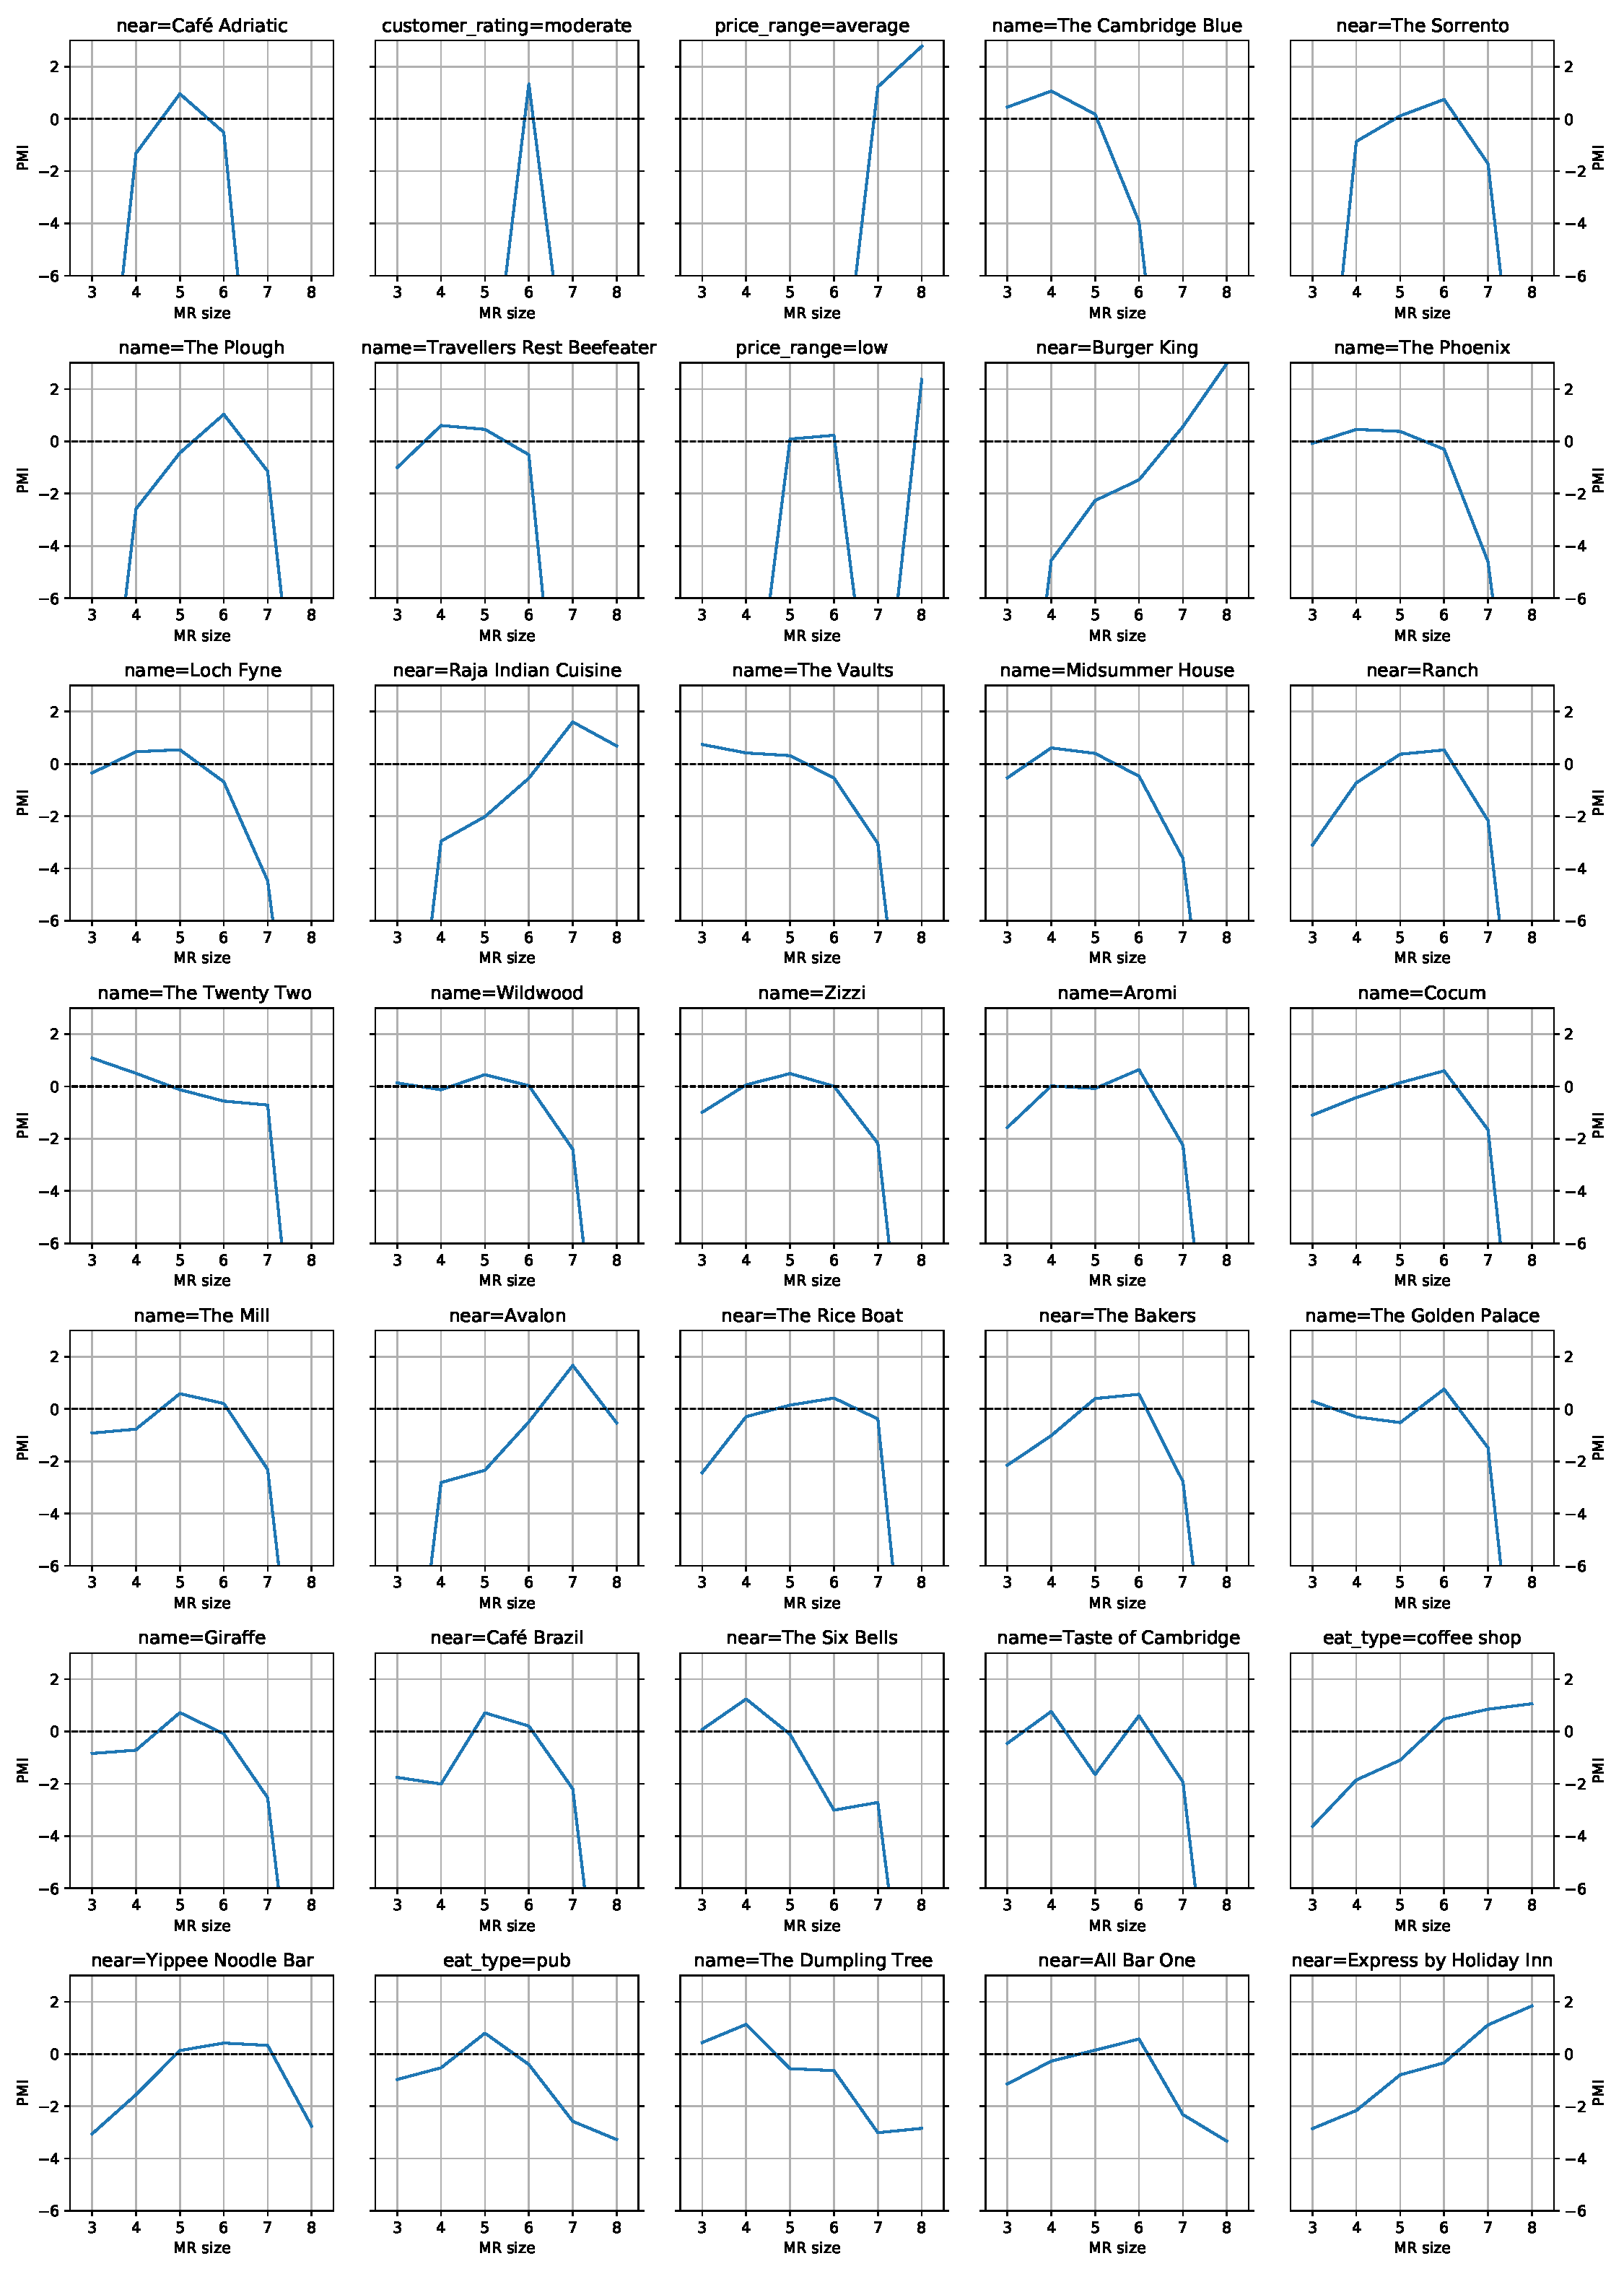
\includegraphics[width=\textwidth]{nlg/trainpmis.pdf}
\end{figure}


\clearpage
\subsection{Data-Augmentation: a Chicken and Egg Problem}

Ideally, we could follow the algorithm  sketched in \autoref{alg:idealda} 
and create synthetic
\meaningrepresentation/utterance pairs to add to our training data.

\begin{algorithm}[t]
$\augdata \gets \{\}$\\
\While{$\setsize{\augdata} < \numSamples$}{
$\tilde{\mr} \sim \daMrDist$ \\
$\boldsymbol{\tilde{\utttoks}} \sim \daUttDist(\boldsymbol{\tilde{\mr}})$\\
%\If{ $\lnot \filter(\tilde{\mr}, \boldsymbol{\tilde{\utttoks}})$}{ $\augdata \gets \augdata \cup \{(\tilde{\mr}, \boldsymbol{\tilde{\utttoks}}) \}$ }
$\augdata \gets \augdata \cup \{(\tilde{\mr}, \boldsymbol{\tilde{\utttoks}}) \}$
}
%    \KwResult{Salience judgements $\bsals = \left[ \bsal_1, \ldots, \bsal_\docSize\right]$}
$\gen_* \gets \operatorname{Train}(\corpus \cup \augdata)$\\
\KwResult{$\gen_*$}
    \caption{Idealized Data Augmentation and Training}
\label{alg:idealda}
\end{algorithm}

If the novel \meaningrepresentations~are drawn from a distribution, 
$\daMrDist$, such that $\daMrDist \ne \corpus_\mr$, 
and the novel utterances are generated from $\daUttDist(\tilde{\mr})$
 such that $\denotes{\boldsymbol{\tilde{\utttoks}}} = \tilde{\mr}$
while maintaining their fluency/naturalness (i.e., $\daUttDist \approx \corpus_\utttoks$),
then 
it is possible that that when training a \sequencetosequence~on the union 
of original training data and synthetic data, the resulting model, $\gen_*$,
 will behave
more systematically, which means more faithfully in our context.

Coming up with a reasonable data-augmentation 
\meaningrepresentation~distribution, $\daMrDist$, is fairly straightforward.
For example we could just sample the size of the \meaningrepresentation, $k$,
uniformly at random, then sample the $k$ \attributes~uniformly at random 
without replacement. Then for each of the attributes, values could be
sampled inversely proportional to their occurrence in the training data, i.e.
\begin{singlespace}
\begin{align*}
\operatorname{count}(a, v) & = \sum_{(\mr, \utttoks) \in \corpus} \mathds{1}\{\AV{$a$}{$v$} \in \mr  \}\\
k & \sim \operatorname{Uniform}(\{3, \ldots, 8\}) \\
p(v|a) & = \frac{\operatorname{count}(a,v)^{-1}}{\sum_{v^\prime \in {\mrvocab}_a}  \operatorname{count}(a,v^\prime)^{-1}} \\
a_i & \sim \operatorname{Uniform}(\{name, \ldots, near, eat\_type\}\setminus\{a_1,\ldots,a_{i-1}\}) & \forall i: i \in  \{1,\ldots, k\}\\
v_i & \sim p(\cdot|a) & \forall i: i \in \{1,\ldots,k\} \\
\tilde{\mr} & = \left[\!\!\left[ 
\begin{array}{c} 
\textsc{Inform} \\
\AV{$a_1$}{$v_1$} \\ \vdots \\ \AV{$a_k$}{$v_k$}  
\end{array}  
\right]\!\!\right]
\end{align*}\end{singlespace}
This procedure should produce valid \meaningrepresentations, and by 
definition $\daMrDist \ne \corpus_\mr$. Additionally, the co-occurance
of an \attribute~and a particular \meaningrepresentation~size will now be 
independent, and the co-occurrance of pairs of attributes will also be independent. 


Unfortunately, it is not clear how we implement utterance distribution
$\daUttDist(\mr)$ since if we had an utterance generation method that could
respond systematically to non-training data distributed \meaningrepresentations, we wouldn't need to perform data augmentation. As a starting point, 
we consider ways of generating samples from a base model $\gen_0$ which 
trained on the available training data, i.e. $\gen_0 = \operatorname{Train}(\corpus)$.

We cannot use $\gen_0$ with beam search as we saw previously,
there are some \meaningrepresentations~that $\gen_0$ won't be able to create utterances for (as we saw with \AV{near}{Burger King}). We could try a variant
of ancestral sampling, however 
it is difficult for ancestral sampling schemes to produce 
extremely different outputs without hurting fluency. 


\subsubsection{Noise Injection Sampling}

The fundamental issue with ancestral sampling is that the randomness of the
model at the word selection stage. This means that in the middle of generating
a phrase it is possible for a disfluent word to be selected, which can
disrupt the current phrase but also destabilize subsequent generation steps
as the model tries to recover from the unsual selection.
Ideally, randomness in a model would occur earlier in determining the 
``topicality'' or ``aboutness'' (you might even say content selection) 
of the generated utterance. Beyond the conditioning input $\ls(\mr)$,
the content that is to be generated is implicitly represented by
inner hidden states of the model. 

In \citet{cho}, they argue that the hidden states, $\decHidState_i$, 
of the \sequencetosequence~decoder lie on a manifold, as a requirement of
the linear separability of the next word prdecition, i.e.
$\gen(\utttok|\utttoks_{1:i},\ls(\mr)) \propto \exp \mathbf{w}_\utttok \cdot \decHidState_i$. The implication is that moving about the manifold will change 
the ``topicality'' of the distribution $\gen(\utttok|\utttoks_{1:i},\ls(\mr))$.
They further suggest adding Gaussian noise to $\decHidState_i$ as a way to
obtain stochastic samples from $\gen$. 

\newtcbox{\stochbox}[1][]{colframe=blue, colback=blue!15, boxrule=0.1mm,
                       nobeforeafter, tcbox raise base, shrink tight, extrude
                       by=0.32mm, #1}
\newtcbox{\detbox}[1][]{colframe=red, colback=red!15, boxrule=0.1mm,
                       nobeforeafter, tcbox raise base, shrink tight, extrude
                       by=0.32mm, #1}


\renewcommand{\algorithmcfname}{Alg.}

\begin{figure}[t]
\begin{center}\small \detbox{Deterministic operation}~~~~\stochbox{Stochastic operation}\end{center}
\resizebox{\textwidth}{!}{%
\begin{minipage}{0.33\textwidth}
\small
\begin{singlespace}
\begin{algorithm}[H]
$\encHidState_{1:\mrSize} \gets \operatorname{enc}(\ls(\mr))$\\
$\predutttok_1 \gets \starttok$\\
$\predutttoks \gets \left[ \predutttok_1\right]$\\
$i \gets 1$\\
\While{$\predutttok_i \ne \stoptok$}{
$\decHidState_i \gets \operatorname{dec}(\predutttoks, \encHidState_{1:\mrSize})$\\
$\vphantom{\boldsymbol{\epsilon_i} \sim \operatorname{Normal}(\zeroEmb, \frac{\sigma}{i})}$\\
\detbox{$\predutttok_{i+1} \gets \argmax_\utttok \gen(\utttok|\decHidState_i)$}\\
$\predutttoks \gets \predutttoks \oplus \left[ \predutttok_{i+1}\right]$\\
$i \gets i + 1$\\
}
%$\gen_* \gets \operatorname{Train}(\corpus \cup \augdata)$\\
\KwResult{$\predutttoks$}
    \caption{\small Greedy Decoding}
%\label{alg:idealda}
\end{algorithm}
\end{singlespace}
\end{minipage}\begin{minipage}{0.33\textwidth}
\small
\begin{singlespace}
\begin{algorithm}[H]
$\encHidState_{1:\mrSize} \gets \operatorname{enc}(\ls(\mr))$\\
$\predutttok_1 \gets \starttok$\\
$\predutttoks \gets \left[ \predutttok_1\right]$\\
$i \gets 1$\\
\While{$\predutttok_i \ne \stoptok$}{
$\decHidState_i \gets \operatorname{dec}(\predutttoks, \encHidState_{1:\mrSize})$\\
$\vphantom{\boldsymbol{\epsilon_i} \sim \operatorname{Normal}(\zeroEmb, \frac{\sigma}{i})}$\\
\stochbox{$\predutttok_{i+1} \sim \vphantom{\argmax_\utttok}\gen(\cdot|\decHidState_i)$}\\
$\predutttoks \gets \predutttoks \oplus \left[ \predutttok_{i+1}\right]$\\
$i \gets i + 1$\\
}
%$\gen_* \gets \operatorname{Train}(\corpus \cup \augdata)$\\
\KwResult{$\predutttoks$}
\caption{\small Ancestral Sampling}
%\label{alg:idealda}
\end{algorithm}
\end{singlespace}
\end{minipage}\begin{minipage}{0.38\textwidth}
\small
\begin{singlespace}
\begin{algorithm}[H]
$\encHidState_{1:\mrSize} \gets \operatorname{enc}(\ls(\mr))$\\
$\predutttok_1 \gets \starttok$\\
$\predutttoks \gets \left[ \predutttok_1\right]$\\
$i \gets 1$\\
\While{$\predutttok_i \ne \stoptok$}{
$\decHidState_i \gets \operatorname{dec}(\predutttoks, \encHidState_{1:\mrSize})$\\
\stochbox{$\boldsymbol{\epsilon_i} \sim \operatorname{Normal}(\zeroEmb, \frac{\sigma}{i})$}\\
\detbox{$\predutttok_{i+1} \gets \argmax_\utttok \gen(\utttok|\decHidState_i + \boldsymbol{\epsilon_i})$}\\
$\predutttoks \gets \predutttoks \oplus \left[ \predutttok_{i+1}\right]$\\
$i \gets i + 1$\\
}
%$\gen_* \gets \operatorname{Train}(\corpus \cup \augdata)$\\
\KwResult{$\predutttoks$}
\caption{\small Noise Injection Sampling}
%\label{alg:idealda}
\end{algorithm}
\end{singlespace}
\end{minipage}
}
\caption{A comparison of greedy decoding, ancestral sampling, and noise injection sampling.}
\label{fig:noiseinj}

%?\begin{minipage}{0.3\textwidth}
%?\begin{singlespace}
%?\begin{algorithm}[H]
%?$\predutttok_1 \gets \starttok$\\
%?$i \gets 1$\\
%?\While{$\predutttok_i \ne \stoptok$}{
%?$\tilde{\mr} \sim \daMrDist$ \\
%?%\If{ $\lnot \filter(\tilde{\mr}, \boldsymbol{\tilde{\utttoks}})$}{ $\augdata \gets \augdata \cup \{(\tilde{\mr}, \boldsymbol{\tilde{\utttoks}}) \}$ }
%?$\augdata \gets \augdata \cup \{(\tilde{\mr}, \boldsymbol{\tilde{\utttoks}}) \}$
%?}
%?%    \KwResult{Salience judgements $\bsals = \left[ \bsal_1, \ldots, \bsal_\docSize\right]$}
%?$\gen_* \gets \operatorname{Train}(\corpus \cup \augdata)$\\
%?\KwResult{$\gen_*$}
%?    \caption{Noise-Injection Sampling}
%?\label{alg:idealda}
%?\end{algorithm}
%?\end{singlespace}
%?\end{minipage}
\end{figure}





We show the noise injection sampling algorithm in \autoref{fig:noiseinj}
along with greedy decoding and ancestral sampling to emphasize the 
how the location of the stochasticity moves from the next word selection (line 8) to a peturbation of the hidden state (line 7). 
Note that in line 7 of the noise injection sampling algorithm, the standard
deviation of the normal distribution, $\frac{\sigma}{i}$, is scaled by the 
decoder step $i$ and in the limit turns to zero, i.e. $\lim_{i \rightarrow +\infty} \decHidState + \boldsymbol{\epsilon}_i = \decHidState$. The inuition 
behind this scaling is that we add the most noise at the first steps 
of decoding, which encourages the decoder to start from a topically novel
region of the hidden state manifold. As the decoding proceeds, the noise
reduces along with the chances of sending the decoder off the manifold
and destabilizing the decoding, and gradually we converge on the behavior of
greedy decoding. 

\begin{table}
    \centering
    \begin{tabular}{c ccc ccc ccc ccc ccc}
        \toprule
        $i$ & 1 & 2 & 3 & 4 &5 & 6 \\
        $\utttok_{i+1}$ &  the  & waterman &is &not& family & friendly \\
        \midrule
        $\gen(\utttok_{i+1}|\decHidState_i; \topkVocab{5}{i})$ & 0.874 & 0.004 & 0.380 & 0.397 & 0.915 & 0.147 \\
    $\gen(\utttok_{i+1}|\decHidState_i; \topkVocab{25}{i})$ &
0.792 & 0.004 & 0.344 & 0.371 & 0.877 & 0.147 \\
     $\gen(\utttok_{i+1}|\decHidState_i; \topkVocab{50}{i})$ &
0.778 & 0.004 & 0.339 & 0.366 & 0.872 & 0.147 \\
       $\gen(\utttok_{i+1}|\decHidState_i; \topkVocab{75}{i})$ &
0.772 & 0.004 & 0.338 & 0.364 & 0.870 & 0.147 \\
        $\gen(\utttok_{i+1}|\decHidState_i; \topkVocab{100}{i})$ & 
0.768 & 0.004 & 0.337 & 0.363 & 0.869 & 0.147 \\
        \midrule
     $\gen(\utttok_{i+1}|\decHidState_i; \nucleusVocab{.95}{i})$     & 
0.796 & 0.000 & 0.352 & 0.377 & 0.909 & 0.148 \\
     $\gen(\utttok_{i+1}|\decHidState_i; \nucleusVocab{.96}{i})$ &
0.789 & 0.000 & 0.349 & 0.374 & 0.898 & 0.148 \\
      $\gen(\utttok_{i+1}|\decHidState_i; \nucleusVocab{.97}{i})$ &
0.781 & 0.000 & 0.345 & 0.370 & 0.892 & 0.148 \\
     $\gen(\utttok_{i+1}|\decHidState_i; \nucleusVocab{.98}{i})$ &
0.773 & 0.000 & 0.342 & 0.367 & 0.882 & 0.148 \\ 
     $\gen(\utttok_{i+1}|\decHidState_i; \nucleusVocab{.99}{i})$ &
0.765 & 0.004 & 0.338 & 0.363 & 0.874 & 0.148 \\
        \midrule
        $\gen(\utttok_{i+1}|\decHidState_i)$ &0.758 & 0.004 & 0.335 & 0.359 & 0.865 & 0.147 \\
        $\gen(\utttok_{i+1}|\decHidState_i + \boldsymbol{\epsilon}_i)$ & 0.321 & 0.170 & 0.408 & 0.489 & 0.785 & 0.514 \\
        \bottomrule
    \end{tabular}

~\\~\\~\\~\\


    \begin{tabular}{c ccc ccc ccc ccc ccc}
        \toprule
        $i$             & 7  & 8 & 9 & 10 & 11 & 12 & 13 & 14 \\
        $\utttok_{i+1}$ &  and &is& located &near& burger & king & . & \stoptok \\
        \midrule
 $\gen(\utttok_{i+1}|\decHidState_i; \topkVocab{5}{i})$ &  0.338 & 0.111 & 0.147 & 0.168 & 0.000 & 0.954 & 0.931 & 0.810 \\
 $\gen(\utttok_{i+1}|\decHidState_i; \topkVocab{25}{i})$ & 0.327 & 0.101 & 0.111 & 0.148 & 0.001 & 0.935 & 0.911 & 0.810 \\
 $\gen(\utttok_{i+1}|\decHidState_i; \topkVocab{50}{i})$ & 0.326 & 0.100 & 0.105 & 0.146 & 0.001 & 0.930 & 0.910 & 0.810 \\
 $\gen(\utttok_{i+1}|\decHidState_i; \topkVocab{75}{i})$    & 0.326 & 0.100 & 0.103 & 0.145 & 0.001 & 0.928 & 0.909 & 0.810 \\
 $\gen(\utttok_{i+1}|\decHidState_i; \topkVocab{100}{i})$ & 0.326 & 0.100 & 0.102 & 0.144 & 0.001 & 0.926 & 0.909 & 0.810 \\
        \midrule
   $\gen(\utttok_{i+1}|\decHidState_i; \nucleusVocab{.95}{i})$      & 0.342 & 0.104 & 0.103 & 0.150 & 0.000 & 0.964 & 0.950 & 0.810 \\
   $\gen(\utttok_{i+1}|\decHidState_i; \nucleusVocab{.96}{i})$ & 0.338 & 0.103 & 0.102 & 0.149 & 0.000 & 0.954 & 0.939 & 0.810 \\
$\gen(\utttok_{i+1}|\decHidState_i; \nucleusVocab{.97}{i})$
     & 0.333 & 0.102 & 0.101 & 0.148 & 0.000 & 0.947 & 0.931 & 0.810 \\
 $\gen(\utttok_{i+1}|\decHidState_i; \nucleusVocab{.98}{i})$   
     & 0.332 & 0.101 & 0.100 & 0.146 & 0.000 & 0.937 & 0.924 & 0.810 \\
 $\gen(\utttok_{i+1}|\decHidState_i; \nucleusVocab{.99}{i})$
     & 0.329 & 0.100 & 0.099 & 0.145 & 0.001 & 0.928 & 0.917 & 0.810 \\
 \midrule
        $\gen(\utttok_{i+1}|\decHidState_i)$ & 0.326 & 0.099 & 0.098 & 0.143 &0.001 & 0.919 & 0.908 & 0.810\\
        $\gen(\utttok_{i+1}|\decHidState_i + \boldsymbol{\epsilon}_i)$ & 0.459 & 0.562 & 0.440 & 0.731 &0.599 & 0.972 & 0.903 & 0.984 \\
 \bottomrule
    \end{tabular}

    \caption{Word selection probabilities when using ancestral sampling,
        top-$k$ sampling (for $k \in \{5,25,50,75,100\}$), 
    nucleus samplling (for $\nucleusthr \in \{0.95, 0.96, 0.97, 0.98, 0.99\}$), and noise-injection sampling ($\sigma = 2.0$).}
    \label{tab:sampprobs}
\end{table}




We can understand noise injection sampling as a compromise between
greedy decoding and ancestral sampling; rather than draw a sequence of utterance
tokens stochasticity, we instead draw a sequence of hidden state spaces.
Given the sequence of hidden state spaces, the corresponding sequence of
utterance tokens is deterministically decided by the most likely next token
given the last hidden state. This next word selection strategy helps to
avoid disfluent continuations.


In \autoref{sample examples}, we show examples of samples obtained with
noise injection sampling as well as some ancestral sampling schemes.
We can see that the ancestral sampling examples are not very diverse,
and occassionally contain disfluencies. The noise injection sampling
example, however, semantically diverges from the input while maintaining
fluency. It was even able to generate an utterance containing the phrase
``near Burger King'' which is was practically impossible to generate with
beam search.


In \autoref{tab:sampprobs}, we show the probability of generating this example
under the various sampling schemes. In our present case, top-$k$ and nucleus
sampling have very similar distributions to the ancestral sampling
distribution ($\gen(\utttok_{i+1}|\decHidState_i)$). All three of these 
techniques assign a very low probability to generating the example utterance,
and in the case of nucleus sampling, it only gives non-zero probability when
using a nucleus of 0.99 cumulative probability (i.e. $\nucleusVocab{.99}{i}$)!
In particular, noise injection sampling puts much more probability 
mass on generating relatively rare \attributevalue~realizations ($i=2$, ``waterman'' and $i=11$, ``burger'').








\subsubsection{Practical Data-Augmentation Scheme}



\newtcbox{\truttbox}[1][]{colframe=green, colback=green!15, boxrule=0.1mm,
                       nobeforeafter, tcbox raise base, shrink tight, extrude
                       by=0.32mm, #1}
\newtcbox{\mrdistbox}[1][]{colframe=orange, colback=orange!15, boxrule=0.1mm,
                       nobeforeafter, tcbox raise base, shrink tight, extrude
                       by=0.32mm, #1}

\newtcbox{\ninjbox}[1][]{colframe=purple, colback=purple!15, boxrule=0.1mm,
                       nobeforeafter, tcbox raise base, shrink tight, extrude
                       by=0.32mm, #1}
\newtcbox{\correctbox}[1][]{colframe=blue, colback=blue!15, boxrule=0.1mm,
                       nobeforeafter, tcbox raise base, shrink tight, extrude
                       by=0.32mm, #1}
\newtcbox{\filterbox}[1][]{colframe=cyan, colback=cyan!15, boxrule=0.1mm,
                       nobeforeafter, tcbox raise base, shrink tight, extrude
                       by=0.32mm, #1}

\newtcbox{\returnbox}[1][]{colframe=violet, colback=violet!15, boxrule=0.1mm,
                       nobeforeafter, tcbox raise base, shrink tight, extrude
                       by=0.32mm, #1}

\begin{figure}[t]
\begin{singlespace}
\begin{algorithm}[H]
\truttbox{$\gen_0 \gets \operatorname{Train}_\utttoks\left(\corpus\right)$} \\
\truttbox{$\dmodel \gets \operatorname{Train}_\mr\left(\corpus\right)$} \\
$\augdata \gets \left\{ \right\}$\\
\While{$\setsize{\augdata} < \numSamples$}{
\mrdistbox{$\samplmr \sim \pdaMrDist$}\\
\ninjbox{$\pdaCandUtts\gets \left\{ \pdaCandUtt \sim 
            \gen_0\left(\cdot|\ls(\samplmr), \pdaCandEps\right) 
            \quad \forall i : i \in \{1,\ldots, k\} \right\} $}\label{lst:pdacand}\\
\ninjbox{$\predutttoks \gets
    \argmax_{\pdaCandUtt \in \pdaCandUtts} 
    \frac{\log \gen_0\left(\pdaCandUtt|\ls(\samplmr),\pdaCandEps \right)}{\setsize{\pdaCandUtt}}$}\label{lst:pdacandselect}\\
\correctbox{$\pdaPredMr \gets \dmodel\left(\predutttoks\right)$}\\
\If{\filterbox{$\lnot \operatorname{Filter}\left(\pdaPredMr, \predutttoks\right)$}}{
    $\augdata \gets \augdata \cup \left\{ \left(\pdaPredMr, \predutttoks\right) \right\}$
}
~\\
}
\returnbox{$\gen_1 \gets \operatorname{Train}_\utttoks(\corpus \cup \augdata)$}\\
\KwResult{$\gen_1$}
    \caption{Data Augmentation with Noise-Injection Sampling and Self-Training }
%\label{alg:idealda}
\end{algorithm}
\end{singlespace}
\caption{A comparison of greedy decoding, ancestral sampling, and noise injection sampling.}
\label{fig:practda}
\end{figure}


Because of its ability to generate semantically divergent and novel
outputs while maintaining fluency, we adopt this noise injection
sampling as our method of sampling utterances, $\daUttDist$, for 
data-augmentation. We show our actual data-augmentation scheme in
\autoref{fig:practda} and now walk through some of the implementation details.

\paragraph{\truttbox{Train base generator $\gen_0$ and \meaningrepresentation~parser $\dmodel$.}}
The algorithm begins by training the base generator, i.e. na{\"i}ve 
\sequencetosequence~model, and \meaningrepresentation~parser $\dmodel$. 
Both models are trained on the same data, with the only real change to the 
$\operatorname{Train}$ sub-routine being which part of a training example
is the ouput and which is the input. Alternatively, $\dmodel$ can 
also be implemented using regular-expression-based rules. We defer detailed 
explanation of $\dmodel$ until the experiments; it suffices to understand
$\dmodel$ as a mapping from utterances to \meaningrepresentations.




\paragraph{\mrdistbox{Sampling a \meaningrepresentation, $\samplmr$}}
Move sampling stuff from above to here.

\paragraph{\ninjbox{Generating a novel utterance with noise-injection 
    sampling.}}
    In \autoref{lst:pdacand} we take $k$ noise-injection samples to construct
    a candidate set of utterances, $\pdaCandUtts$. From $\pdaCandUtts$ we
    select as our noise-injection sample, the utterance $\predutttoks$
    which has the highest average token log-likelihood (\autoref{lst:pdacandselect}). We do this selection step so as to be extra cautious and avoid adding
    any potentially disfluent utterance. 
    
    \paragraph{\correctbox{Predict \meaningrepresentation~$\pdaPredMr$ from
    $\predutttoks$.}} Because the noise-injection sampling produces highly
semanticly deivergent utterances, it is unlikely that $\denotes{\predutttoks } = \samplmr$. Instead we use the \meaningrepresentation~parser, $\dmodel$, to
recover the most likely \meaningrepresentation, $\pdaPredMr = \dmodel\left(\predutttoks\right)$.

\paragraph{\filterbox{Check synthetic datapoint $(\pdaPredMr,\predutttoks)$.}}
We do one last quality check on the synthetic example $(\pdaPredMr,\predutttoks)$ before adding it to the augmented dataset, $\augdata$. We make sure that
the probability of $\pdaPredMr$ under $\dmodel$ is above a threshold when using
a model-based \meaningrepresentation~parser. When using a rule-based
\meaningrepresentation~parser, we check to make sure that there are no
repeated \attributevalue-pairs in $\predutttoks$, e.g., ``Aromi is a 
coffee shop and it is a coffee shop.'' If the \meaningrepresentation/utterance
pair passes these final quality checks, we add it to $\augdata$.

\paragraph{\returnbox{Train an augmented generator $\gen_1$ on $\corpus \cup \augdata$.}} After generating a dataset of synthetic data, we train a new 
generation model, $\gen_1$, on the union of the original training data
and the newly generated synthetic data. We refer to this model as 
the augmented generator and as we will show empirically, the augmented
model is more faithful than the base generator, $\gen_0$.
We call this process self-training because the $\gen_1$ and $\gen_0$ share 
the same architecture, and $\gen_1$ is trained on data produced by $\gen_0$.

\section{Experiments}

We experimentally validate the noise-injection sampling and self-training
data-augmentation scheme on the E2E Challenge dataset~\citep{something} 
and the Laptops and TVs datasets \citep{wen}, three collections of 
\meaningrepresentation/utterance pairs for training response generation models

\naturallanguagegeneration~models for t

\subsection{Datasets}

We use three recent dialogue generation datasets in our experiments,
the E2E Challenge Dataset \cite{duvsek2019evaluating}, and the Laptops and 
TVs datasets \cite{wen2016multi}.
We only briefly review them here.
Each dataset consists of \meaningrepresentations~paired with one or more 
reference utterances.
%(see \autoref{figure:introexample} for an example from the E2E dataset).
%The structure of each \meaningrepresentation~is relatively simple, 
%consisting of the 
%dialog act itself, (e.g. \textit{inform}, \textit{recommend}, 
%\textit{compare}, etc.) and a variable number of attribute slots
%which need to be realised in the utterance. 
All attribute values 
come from a closed vocabulary.
%If an attribute is not present in the MR it should not be realized in the 
%corresponding utterance. 

The three datasets also represent different training size conditions; 
with the E2E Challenge dataset representing the ``large data'' training
condition and the Laptops and TVs dataset representing ``small data'' conditinos. See \autoref{datasizes} for dataset size statistics.
The E2E Challenge dataset has only one dialogue act, \textsc{Inform}, 
and its training \meaningrepresentations~contain three to eight
\attributes~unique attributes. 
The Laptops and TVs datasets contain a more diverse set of \meaningrepresentation/utterance pairs. There are {\color{red}???} unique dialogue acts. 
The number of minimum and maximum \attributes~varies according to the dialogue
act. See \autoref{avdeets} for detailed statistics of the dialogue acts
and \attributevalue~pairs for the three training sets. 


\paragraph{Delexicalization}
Prior work using neural \naturallanguagegeneration~models often relies on 
delexicalization, that is, replacing realizations of named-entity or 
numeric values in an utterance with a placeholder token, in order to alleviate
data sparsity issues and yield better generalization when a generating utterances about named-entities not seen in the trianinig dataset. For example
on the E2E Challenge dataset, the \Atr{name}~and \Atr{near}~attributes
are often delexicalized because they are proper names of estabilishments
that are simple to find and replace in the utterance.

For example, the fully lexicalized utterance 

\begin{center}\noindent~~~~\textit{Near The Six Bells is a venue that is children
friendly named The Golden Curry.}\end{center}

\noindent can be delexicalized as

\begin{center}\noindent ~~~~\textit{Near <<near>> is a venue that is children
friendly named <<name>>.}\end{center}

Delexicalized utterances can be re-lexicalized as a post-processing
step, where the placeholder token is replaced with the correct value text.

On the E2E Challenge dataset, we experiment with delexicalization of the 
\textit{Name} and \textit{Near} attributes since thah have a relatively large vocabulary of valid slot fillers, some of which are only seen  infrequently in the training data;
it can be difficult for fully lexicalized models to produce some of the 
rarer location names for these attributes. 

However, since delexicalization might be difficult or 
impossible in other domains, we implement both delexicalized and lexicalized
versions of the generation models on the E2E dataset to 
more fully evaluate the
self-training method.
   

The evaluation script for the Laptops and TVs datasets uses delexicalization
to evaluate attribute realization error, and so we use it here to be 
consistent with prior work, 
delexicalizing all possible attributes.
%



\subsection{Generation Models}

We use a two-layer, unidirectional GRU architecture with Bahdanau style
attention for our 
\sequencetosequence~model. We set $\embDim = \hidDim = \encDim = \decDim = 512$, that is, we use 512-dimensional embedding and hidden states.

We fit model parameters, $\params$, by minimizing the negative log-likelihood
of the training set, $\corpus$, i.e. $\mathcal{L}(\params) = - \sum_{(\mr, \utttoks) \in \corpus  }  \log \gen\left(\utttoks|\ls(\mr);\params\right).$
When generating utterances for evaluation (i.e. not for use in noise-injection sampling) we use either greedy decoder or beam decoding with a 
beam size of eight.
The beam search terminates after eight candidates have been generated;
the candidates are reranked by average token log-likelihood, $\frac{\log \gen\left(\utttoks|\ls(\mr)\right)}{\setsize{\utttoks}}$. In these experiments, we \textbf{do not} use a discriminative reranker to ensure the faithfulness of the 
selected beam candidate. 

\subsection{\MeaningRepresentation~Parsing Models}

Given a novel utterance $\predutttoks$~sampled from $\gen$, we need to 
reliably parse the implied \meaningrepresentation, i.e. 
$\pdaPredMr = \dmodel(\predutttoks)$, 
where \dmodel~is our parsing model. We have two things going for us in 
our experimental setting. First, even with noise injection sampling,
model outputs are fairly patterned, reducing the variability of the utterances
we need to parse in practice. 

Second, the \meaningrepresentation~in this study are
flat lists of attributes that are somewhat independent of each other.
We only need to detect the presence of each attribute and its value.
For the Laptops and TVs datasets we also need to recover the dialog
act but these also are signaled by a fairly limited repertoire 
of cues, e.g. ``we recommend.'' % or ``compared to'' for the 
%\textit{Recommend} and \textit{Compare} DAs respectively. 
Given this, we experiment with both hand crafted regular expression 
rules and learned classifiers to predict the value of
an attribute if present or that it is missing. 


\paragraph{Rule-based parser (\ruledmodel)} We design hand-crafted 
regular expression based rules to match for the presence of key phrases 
for each of the attributes and DAs in the datasets while also checking to
make sure that there is only one match per attribute.

To construct the rules, we look through both the training data references as 
well as the generation model outputs as this is what the rules will
be operating on in practice. For each lexicalized attribute (and DA) we 
develop a list of regular expressions % or conjunctions of regular expressions
such as,
\texttt{/is (family|kid|child) friendly/} $\Rightarrow$ \textit{familyFriendly[yes]}.
For the delexicalized attributes, we simply check for the presence 
of the placeholder token. 

%One failure mode of the generation models on
%Laptops and TVs is to use the wrong attribute value token in an expression,
%e.g. ``...has a DRIVESIZERANGE price range,'' so we add additional rules
%to mark an utterance/MR pair as invalid in these cases.
%e.g.
%\begin{align*}
%\texttt{/price/}~\land~\lnot\texttt{/PRICERANGE/} 
%    \Rightarrow \emptyset.
%\end{align*}

We design these rules to be high precision, as it is safer to miss out on 
more obscure varieties of utterance to avoid adding incorrectly parsed data 
points.
However,  in many cases the rules are also high recall as well. 
The average F-score on the E2E validation set is 0.93.
%In some cases, this is probably
%close to the performance ceiling; the human authored references in the validation
%set are noisy and are often incorrectly labeled or omit realizing attributes.


%This is a relativity conservative approach as it is possible we will
%miss good phrases, however, it is more important that we add as little
%noise to augmented dataset as possible.
%rules to detect the presence of 
%key phrases related to each attribute's realization. We design these rules
%to be high-precision, so even while we may not cover all possible 
%only need to augment our training data with pairs $(\samplex, \sampley)$ 
%If the rules indicate that the MR is valid (e.g. only mentions an attribute
%once). While we may miss out on more diverse constructions, we more reliably
%ensure the augmented data is correct, i.e. \sampley~correct conveys the
%discourse act and attibute values specified in \samplex. Adding too many
%incorrect pairs will degrade the reliability of our final generation model.



\paragraph{Classifier-based parser (\learndmodel)} 
It is perhaps too optimistic to believe we can construct reasonable rules
in all cases. Rule creation quickly becomes tedious and for more complex
MRs this would become a bottleneck. To address these concerns, we also 
study the feasibility of using learned classifiers to predict the presence
and value of the attributes. For each attribute in the E2E dataset,
we trained a separate convolutional neural network (CNN) classifier 
to predict the correct attribute value (or \textit{n/a} if the attribute is 
not present).
The CNN architecture follows that of \citet{kim2014convolutional} and is 
trained with 
gradient descent on the original training data. 



We use a separate CNN classifier for each attribute to predict
the corresponding value (or \textit{n/a}) from an utterance $\utttoks$.
We first look up the tokens in $\utttoks$ in an embedding matrix $E$
to obtain a matrix $W\in\mathbb{R}^{N \times D}$ where $D=50$ is
the embedding dimension.

We then apply a series of unigram, bigram, and trigram convolutional
filters each with $50$ output features.
After concatenating and max-pooling over the sequence dimension,
and applying a ReLU activation,
we obtain a hidden layer in $\mathbb{R}^{150}$.
We then apply another fully-connected layer with ReLU activation
which down projects the hidden layer to $\mathbf{R}^{50}$.
Finaly we apply the final softmax layer to predict the class label.

During training we apply dropout (with drop rate 0.25) to 
the embedding layer, convolutional filter outputs, and hidden
layers. We train for 30 epochs with gradient descent
using  a learning rate of 0.25 and 
weight decay penalty of 0.0001, using validation set F1
as our model selection criterion.
The average E2E validation F-score is 0.94.
%iThe classifiers
%required significantly less manual effort
%(and almost zero domain knowledge) to construct.

\subsection{E2E Challenge Self-Training Experiments}
 We train base generators $\basegen$~on the original training data $\corpus$, 
 with and without
delexicalizing the \textit{Name} and \textit{Near} attributes. 
We train for 500 epochs with gradient descent. We use a batch size of 128,
with a learning rate of 0.25, weight decay penalty of 0.0001, and a dropout 
probability of 0.25.
We select the best model iteration using validation
set BLEU score\footnote{We use the official shared task script to
compute automatic quality metrics on the E2E dataset.}.

Using the self-training method outlined in \autoref{section:selftrain},
we create augmented datasets using either $\learndmodel$~or
$\learndmodel$, which we refer to as 
$\augdata_{\ruledmodel}$ and $\augdata_{\learndmodel}$ respectively 
($\learndmodel$~is only in the delexicalized setting).

To sample a novel MR with  $S$ attributes, we sample a combination of $S-1$ attributes
uniformly at random %from the $\binom{7}{S-1}$ possible combinations
(always appending the \textit{name} attribute since every MR contains it).
 We 
then sample attribute values for each slot % independently
inversely proportional to their empirical frequency
in the training set so as to increase the likelihood of creating a novel
or under-represented MR.


After obtaining such a sample $\utttoks$~we then perform noise injection sampling,
generating 200 samples $\pdaCandUtt \sim 
\basegen(\cdot|\utttoks, \epsilon^{(i)})$ 
in parallel and discarding all but the top 20
samples by average log likelihood according to $\basegen$.
We also discard any utterances that have previously been generated.
%to avoid 
%adding repeat utterances to the augmented data.

We then apply the parser to the sampled utterances, to obtain its
predicted MR, $\pdaPredMr^{(i)} = \dmodel(\pdaCandUtt)$. If using 
the rule based parser $\ruledmodel$~and $\pdaPredMr^{(i)} 
= \emptyset$, i.e. the utterance
does not have a valid parse, we discard it.
Similarly, when using the classifier based parser, \learndmodel, if 
any attribute value is predicted with less than 50\% probability we discard 
it. All surviving $(\pdaPredMr^{(i)}, \predutttoks^{(i)})$ pairs are added to \augdata.
We repeat this process 25,000 times for each valid MR size $S$.
See \autoref{table:samplequal} for statistics on the total sample sizes 
after filtering.
%yielding 1,591,788 additional samples for the lexicalized \basegen/\ruleclf,
%501,909 for the delexicalized \basegen/\ruleclf, and 384,436 for the 
%delexicalized \basegen/\learnedclf~pairings.

\

For both $\corpus \cup \augdata_{\ruledmodel}$ and 
$\corpus \cup \augdata_{\learndmodel}$ we train new generators \auggen~using 
the same training setting as above (although we terminate training after 50 
epochs
because the models converge much faster with the additional data).

We report BLEU, ROUGE-L, and METEOR on the E2E test set.
We show results for both greedy and beam decoding with beam size 8
under $\basegen$~and
\auggen~models. We compare our models to the best sequence-to-sequence DNN
model, Slug \cite{juraskaslug2slug}, the best grammar rule based model, 
DANGNT \cite{nguyen2018structurebased},
and the best template based model, TUDA \cite{puzikov2018e2e}, as determined during 
the shared task evaluation \cite{duvsek2019evaluating}.


%We then create augmented datasets using the methods
%described in section~\ref{}, using either the rule-based classifier 
%\ruleclf~or learned classifier \learnedclf~to reconstruct the MRs.
%For each filtering method we train a new generator \auggen~on the union of 
%the original training data the augmented data collection, i.e. 
%$\trdata \cup \augdata^{\ruleclf}$ and $\trdata \cup \augdata^{\learnedclf}$.
%The architecture of \auggen ~ is identical to that of \basegen. We 
%train \auggen ~ for 50 epochs (with the added data, the \auggen ~ 
%models converge much faster), again selecting the best model via validation 
%set BLEU score.

\subsection{Laptops and TVs Self-Training}
We perform similar experiments on the Laptops and TVs datasets. 
We train a separate \basegen~model for each dataset 
for 300 epochs with a learning rate of 0.1
for Laptops and 0.25 for TVs. The weight decay penalty was 0.0001 
and dropout probability was 0.25. Best model iteration is determined
by validation set BLEU score. As in the E2E experiments, we create an augmented
dataset for both the Laptops and TVs dataset using the method
outlined in \autoref{section:selftrain}. We then train new generators 
\auggen~on the union of original training data and the augmented dataset.

On the Laptops and TVs dataset,
%each DA can have a different minimum and maximum number of attributes.
for each DA and legal number of attributes $S$ we draw $S$ random attributes
(modulo any required attributes like \textit{Name}; not all DAs require it).\footnote{A number of attributes $S$ is ``legal'' if we observe a DA instance with that 
many attributes in the original training data.}
%For binary attributes, or attributes that can have the \textit{don't care}
%value, we randomly sample these values, to obtain a MR \mrx.

We then perform noise injection sampling,
generating 200 samples $\pdaCandUtt \sim 
\basegen(\cdot|\mrtoks, \epsilon^{(i)})$ under the same settings as the E2E
dataset. We repeat this process 25,000 times for each DA and DA size.
We obtain 373,468 and 33,478 additional samples for the Laptops 
and TVs datasets respectively.


We automatically evaluate our models using the evaluation script of
\citet{wen2016multi}, which computes BLEU scores, as well as slot
alignment error rate (since this dataset is almost fully delexicalized,
it simply checks for the presence of the correct attribute placeholders
according to the MR). We compare again to the Slug model as well
as the Semantically Conditioned LSTM (SCLSTM) \cite{wen2015semantically}
which report state-of-the-art results on these datasets.


\begin{table}
\centering
\begin{tabular}{rcccc}
\toprule
Model  & BLEU & R.-L & MET. \\ \midrule
Slug   & 66.19 & 67.72 & 44.54  \\  
DANGNT & 59.90 & 66.34  & 43.46  \\
TUDA   & 56.57 & 66.14  & 45.29  \\
        \midrule
delex. \basegen~~~~~~greedy & 66.91 & 68.27 & 44.95 \\
                      beam & \textbf{67.13} &  \textbf{68.91} &  45.15  \\
        \auggen~\ruleclf~greedy   &  65.57 & 67.71 & 45.56  \\
                             beam & 66.28 &  68.08 &  \textbf{45.78}  \\
     \learnedclf~greedy & 63.76 &  67.31 &  44.94  \\
   beam   & 
 64.23 &  67.54 &  45.17  \\
\midrule
   lex. \basegen~~~~~~greedy & 60.35 &  64.51 & 41.82  \\
                      beam   & 61.81 &  65.83 & 42.69  \\
    \auggen~\ruleclf~greedy & 64.74 &  68.21 & 44.46  \\
       beam & 64.81 &  67.83 &    44.39  \\
\bottomrule
\end{tabular}
\caption{BLEU, ROUGE-L, and METEOR metrics on the E2E test set. Baseline methods all rely
on at least partial delexicalization, puting our lexicalized models at a relative disadvantage.}

\label{table:autoqual}
\end{table}





\begin{table*}
\setlength{\tabcolsep}{5pt}
\center
  \begin{tabular}{rrrr ccccc ccc ccc}
    \toprule
 \multicolumn{4}{c}{
\multirow{2}{*}{
Model} }
       & \multirow{2}{*}{Name} & \multirow{2}{*}{Near}    
            &  Family  & 
           \multirow{2}{*}{Area}    & Customer & \multirow{2}{*}{Food} 
      & Price & Eat & \multirow{2}{*}{All} \\
  & & & &  &  & Friendly & 
        & Rating &  & Range & Type &  \\
\midrule
\multicolumn{4}{r}{Slug}  
                    & 0 & 0 & 6  & 1  & 6  &  10  & 35  & 9  & 67 \\ 
\multicolumn{4}{r}{DANGNT}
                    & 0 & 0 & 18  & 0  & 0  & 0  & 0  & 58  & 76 \\ 
\multicolumn{4}{r}{TUDA}  
                    & 0 & 0 & 0  & 0  & 0  & 0  & 0  & 0    & \textbf{0} \\
\midrule
delex. & \basegen & & greedy 
                    & 0   & 0   & 23 & 23 & 16 & 26 & 27 & 0 & 115 \\ 
& & & beam          & 0   & 0   & 60 & 3  & 9  & 3  & 8  & 0 & 83  \\ 
& \auggen & \ruledmodel & greedy 
                    & 0   & 0   & 0  & 0  & 0  & 0  & 0  & 0 & \textbf{0} \\ 
 & & & beam         & 0   & 0   & 0  & 0  & 0  & 0  & 0  & 0 & \textbf{0} \\
 & & \learndmodel & greedy 
                    & 0   & 0   & 1  & 0  & 8  & 1  & 9  & 0 & 19 \\
 & &  & beam        & 0   & 0   & 0  & 0  & 3  & 0  & 0  & 0 & 3 \\
\midrule
lex. & \basegen & & greedy 
                    & 145 & 141 & 14 & 15 & 2   & 14 & 2  & 0 & 333 \\
 & & & beam         & 155 & 124 & 62 & 0  & 0   & 0  & 0  & 0 & 341 \\ 
 & \auggen & \ruledmodel  & greedy 
                    & 0   & 0   & 2  & 0  & 0  & 125 & 0  & 0 & 127 \\
&  &  & beam        & 0   & 2   & 0  & 0  & 0  & 119 & 0  & 0 & 121 \\
\bottomrule
    \end{tabular}
\caption{Attribute realization errors on the E2E test set. The Slug model and our delexicalized models delexicalize the NAME and NEAR slots, 
    thus making 0 errors on these attributes. DANGNT and TUDA models perform complete delexicalization. } 
\label{table:autosem}
\end{table*}






\subsection{E2E Challenge Results}

Surprisingly, \basegen~using greedy decoding surpases all of the 
baseline systems. This is quite shocking as the Slug model ensembles
three different sequence-to-sequence models producing 10 outputs each using beam search and reranking based on slot alignment to select the final generation
output. The $\auggen$/$\ruledmodel$~model remains competitive with Slug, 
again even using greedy decoding.
The $\auggen$/$\learndmodel$~starts underperforming Slug on BLEU score but
remains competitive on ROUGE-L and METEOR again when using greedy decoding.
Overall the augmented training data tends to hurt generation quality.
In this regard, the added noise of the trained classifier exacerbates things
as it reduces quality more than the rule-based filtering. 

In the lexicalized setting,
$\basegen$~produces lower quality output than the Slug system.
However, the augmented training procedure increases
the quality of the lexicalized $\auggen$~model which beats Slug on ROUGE-L.


The automatic quality evaluations are somewhat limited, however. To gain
more insight into model performance
we apply our rule based parser to estimate attribute realization error
for all system outputs on the test set,
similarly to \cite{duvsek2019evaluating}
(e.g., if the MR specifies \textit{food[French]},
we check to make sure the generated utterance says so). 
The results of this evaluation are shown in \autoref{table:autosem}.
Immediately, it is revealed that \basegen~is far worse than the baseline 
methods making 115 and 83 errors using greedy and beam decoding respectively.


The $\auggen$/$\ruledmodel$~model achieves zero test set
errors even when using the greedy 
decoding. The $\auggen$/$\learndmodel$~model is slightly worse (in agreement 
with the automatic quality measurements), but its greedy search is still
superior to the more sophisticated Slug decoder, achieving 19 total
test set errors compared to Slug's 67 errors.



The lexicalized $\basegen$~model has especially high error rates, 
particularly on the \textit{Name} and \textit{Near} attributes.
With augmented data training, the $\auggen$~model reduces these errors
 to zero when using greedy search and 2 with beam search. Unfortunately,
the augmented training is more unstable in the lexicalized setting, 
as it produces a large spike in \textit{food} attribute errors, although
the $\auggen$~models still have lower overall error than  $\basegen$.


\subsection{Laptops and TVs Results}
The results are more mixed here. Our BLEU scores are about 15 points 
below the baselines on the Laptops dataset and 20 points below the 
baselines on the TVs dataset. 
Upon examing  the evaluation script in detail we see that 
BLEU score is calculated using 5 model outputs which \citet{juraskaslug2slug}
and \citet{wen2016multi} do. We only produce the 1-best output
at test time,
perhaps explaining the difference.

Looking through our model
outputs we see mostly good utterances, often nearly exactly matching the 
references.
Our models outperform the state of the art models on errors. The best state of the art models  make errors by generating sentences that do not match the input representation 0.79\%  and 1.67\% of the time on the Laptops and TVs datasets
respectively. Our \auggen~model reduces that error to only 0.13\% and 
0.20\%.

%We do achieve the lowest error rates, with \auggen~beam
%decoding achieving a 0.2\% error rate versus the previous best of 1.67\%
%on the TVs dataset, and \auggen~greedy decoding achieving a 0.13\% error
%rate compared the 0.79\% baseline rate.



\begin{table}
    \begin{tabular}{lrrrr}
        \toprule
        & \multicolumn{2}{c}{Laptops} & \multicolumn{2}{c}{TVs} \\
        Model & BLEU & Err. & BLEU & Err.  \\
        \midrule
        SCLSTM    & 51.16 &   0.79\% & \textbf{52.65} &   2.31\%\\
        Slug & \textbf{52.38}  &  1.55\% & 52.26  &  1.67\% \\
        \basegen~~beam  &37.13  &0.72\% & 32.63 & 0.72\% \\
        \auggen~~greedy & 37.21 &  \textbf{0.13\%} & 32.43 & 0.28\%\\
        ~~~~~~beam   & 37.19 & 0.14\% & 32.59 &  \textbf{0.20\%} \\
\bottomrule
    \end{tabular}

    \caption{BLEU and automatic attribute error on the Laptops and TVs
    datasets.}
    \label{table:laptoptvautoqual}
\end{table}


\subsection{Experiment Human Evaluation} 

\paragraph{E2E Dataset} We had two undergraduate students not involved with 
the research look at 100 random test set utterances for six
of our model variants. They were shown
both the Slug output and one of our model outputs and asked to select
which output was of better linguistic quality and correctness or 
indicate that they were equally good.
 We resolved disagreements in favor of the baseline,
i.e. if any annotator thought the baseline was better we considered it so.
If an annotator marked one of our 
systems as better and the other marked it as equal, we considered it 
equal to the baseline. Inter-annotator agreement was high, with 92\% agreement on correctness
and 88\% agreement on quality.

\autoref{humane2e} shows the results of the evaluation.
We find that the \auggen~model outputs are indistinguishable from the Slug
model in terms of linguistic quality, regardless of the setting.
In terms of correctness, the lexicalized \auggen~model is as good as or better than the Slug model 98\%
of the time. 
%We again stress that the \auggen~model only uses beam search 
%with beam size 8, while Slug is delexicalized, and consists of an ensemble of 
%three DNN models each producing 10 outputs via beam search, and reranking 
%to select the candidate that minimizes attribute realization error.
When using the delexicalized models, we don't even need beam search.
The delexicalized \auggen~greedy decoder is as good as or better 
than Slug 100\% of the time.

\paragraph{Laptops Dataset} We had the same annotators look at 100 random 
\textit{Inform}
DAs from the Laptops test set since they are the majority DA type and we 
could use the same annotator
guidelines from the E2E experiment. We do not have access to the Slug
or SCLSTM outputs on this dataset, so we compared to one of the two
test set reference sentences (picking at random) vs. 
the $\auggen$/$\ruledmodel$~with greedy decoding. \autoref{humanlaptop}
shows the results. Despite the low BLEU scores, we find our outputs
to be of comparable quality to references 91\% of the time. Moreover,
they are equally as correct as the human references 100\% of the time.
Annotators agreed 99\% and 87\% of the time on correctness and quality 
respectively.


\begin{table}
\center
    \begin{tabular}{r ccc| ccc}
\toprule
        & \multicolumn{3}{c}{Correct.} & \multicolumn{3}{c}{Quality} \\
    Model & $>$ & $=$ & $<$ & $>$ & $=$ & $<$ \\
\midrule
delex.~\basegen~b & 7 & 89 & 4 & 1 & 96 & 3 \\
delex.~\auggen~\ruledmodel~g & 7 & 93 & 0 & 0 & 100 & 0 \\
delex.~\auggen~\ruledmodel~b & 7 & 93 & 0 & 0 & 100 & 0 \\
delex.~\auggen~\learndmodel~g & 5 & 95 & 0 & 0 & 100 & 0 \\
delex.~\auggen~\learndmodel~b & 8 & 92 & 0 & 0 & 100 & 0 \\
lex.~\auggen~\ruledmodel~g & 8 & 90 & 2 & 0 & 100 & 0 \\
\bottomrule
\end{tabular}
\caption{Human correctness and quality judgments (\%). Comparisons are better
than ($>$), equal to ($=$), and worse than ($<$) the baseline Slug model.
(g) and (b) indicate greedy and beam decoding respectively.}
\label{humane2e}
\end{table}

\begin{table}
    \center
    \begin{tabular}{c ccc| ccc}
\toprule
        & \multicolumn{3}{c}{Correct.} & \multicolumn{3}{c}{Quality} \\
    Model & $>$ & $=$ & $<$ & $>$ & $=$ & $<$ \\
\midrule
delex. \auggen~\ruledmodel~g & 0 & 100 & 0 & 2 & 91 & 7 \\

\bottomrule
\end{tabular}
\caption{Human correctness and quality judgments (\%). Comparisons are better
than ($>$), equal to ($=$), and worse than ($<$) the test set references.}
\label{humanlaptop}
\end{table}

  %"A": Path("base_delex_beam.tsv"),

%4 2 44
%1 3 46

    %"B": Path("aug_rule_delex_greedy.tsv"),
%4 0 46
%0 0 50


%    "C": Path("aug_rule_delex_beam.tsv"),
%4 1 45
%0 0 50


%    "D": Path("aug_clf_delex_greedy.tsv"),
%1 1 48
%0 0 50


%    "E": Path("aug_clf_delex_beam.tsv"),
%5 1 44
%0 0 50


%    "F": Path("aug_rule_lex_beam.tsv"),
%6 1 43
%0 0 50





\subsection{Analysis}

We hypothesize that self-training improves the correctness of outputs
by sacrificing some expressivity of the model. For example, 
\auggen~BLEU scores
on the E2E dataset drop by at least 0.8 as compared to \basegen~with beam
search. We see a similar pattern on the TVs dataset. Self-training
increases automatic metrics in the lexicalized setting, but this could 
be attributable to reductions  in \textit{Name} and \textit{Near}
realization errors, which are orthogonal to the 
syntactic diversity of generation.

To better quantify these effects we report the average length in words, 
average number of sentences, and average revised Developmental Level (D-Level)
score according to the D-Level analyser \cite{lu2009automatic}.
The D-Level analyser automatically categorizes the syntactic complexities 
of an utterance into one of eight categories, with eight being the most
complex, based on the revised Developmental Level scale \cite{rosenberg1987indicators,covington2006complex}.


\autoref{table:samplequal} shows the statistics for the E2E test set outputs. 
In the lexicalized setting, the mean D-level results support our hypothesis;
syntactic complexity of test set outputs decreases from $\basegen$~to~$\auggen$.
In the delexicalized setting this is somewhat true; three of 
the $\auggen$~models have lower mean D-level scores than $\basegen$~with 
greedy decoding. Curiously, $\auggen$/$\learndmodel$~with beam search has the 
highest overall syntactic complexity of any our model variants, at odds
with our hypothesis.
No models are as syntactically complex as the human references, but our
models come closest, with a mean D-Level category of 1.87 using the delex. $\auggen$/$\learndmodel$~model with beam decoder. %, compared to 1.39 with Slug. 


We  also 
see that $\auggen$/$\ruledmodel$~models %are on average two words longer than
%the human references and Slug outputs. Additionally they 
are over two sentences
in length on average while the human references are under two sentences,
suggesting they are more often falling back to simple but reliable
ways to realize attributes (e.g., appending ``It is a family-friendly venue.'').

\begin{table}[t]
    \begin{tabular}{llll}
    \toprule
    Model & Words & Sents & MDL \\
    \midrule
    Human Refs. & 24.06& 1.76& \textbf{2.25}\\
    Slug &24.20 &1.86 & 1.39 \\
    \midrule
    lex. \basegen~greedy &25.73 &2.18 & \textbf{1.84} \\
    lex. \basegen~beam   &26.00 &2.20 & 1.50 \\
    lex. \auggen~\ruledmodel~greedy & 26.01& 2.20& 1.39 \\
    lex. \auggen~\ruledmodel~beam   & 26.04&2.17 & 1.45 \\
    \midrule
    delex. \basegen~greedy & 24.83& 2.10 & 1.79 \\
    delex. \basegen~beam &24.51 & 2.03 & 1.48 \\
    delex. \auggen~\ruledmodel~greedy & 26.50 & 2.29 & 1.74 \\
    delex. \auggen~\ruledmodel~beam & 26.46 & 2.28 & 1.74 \\
    delex. \auggen~\learndmodel~greedy & 25.33&1.76 & 1.77 \\
    delex. \auggen~\learndmodel~beam &25.49 &1.75 & \textbf{1.87} \\
    \bottomrule
    \end{tabular}
    \caption{Words/sentences per utterance
    and mean D-Level score of model outputs on the E2E dataset.}
\end{table}

% \basegen~delex~greedy & 24.8 &2.1 & 1.79 \\  
%                    \basegen~delex~beam &24.5 &2.0 & 1.49 \\
%            \auggen~\ruleclf~delex~greedy & 26.5 & 2.3 & 1.74  \\
%            \auggen~\ruleclf~delex~beam &26.5 &2.3 & 1.74 \\
%         \auggen~\learnedclf~delex~greedy & 25.3& 1.8& 1.77\\
%         \auggen~\learnedclf~delex~beam & 25.5 & 1.7 & 3.76\\
%\midrule
%                    \basegen~lex~greedy & 25.7& 2.2& 1.84 \\  
%                    \basegen~lex~beam & 26.0& 2.2& 1.50 \\
%            \auggen~\ruleclf~lex~greedy & 26.0&2.2 &1.39 \\
%            \auggen~\ruleclf~lex~beam & 26.0&2.2 & 1.45 \\
%
%    \end{tabular}
%\end{table*}

%human_test
%Filename, Sentences, Level0, Level1, Level2, Level3, Level4, Level5, Level6, Level7, MeanLevel
%human.parses.m2, 8261, 3625, 7, 1212, 1627, 195, 224, 222, 1149, 2.25
%slug_test
%Filename, Sentences, Level0, Level1, Level2, Level3, Level4, Level5, Level6, Level7, MeanLevel
%parse.txt, 1159, 753, 0, 152, 103, 19, 0, 0, 132, 1.39
%
%e2e.base.lex.greedy.test
%Filename, Sentences, Level0, Level1, Level2, Level3, Level4, Level5, Level6, Level7, MeanLevel
%parse.txt, 1373, 689, 0, 241, 241, 30, 0, 6, 166, 1.84
%e2e.base.lex.beam.test
%Filename, Sentences, Level0, Level1, Level2, Level3, Level4, Level5, Level6, Level7, MeanLevel
%parse.txt, 1386, 820, 0, 182, 213, 41, 2, 0, 128, 1.50
%
%e2e.aug.rule.lex.greedy.test
%Filename, Sentences, Level0, Level1, Level2, Level3, Level4, Level5, Level6, Level7, MeanLevel
%parse.txt, 1384, 849, 0, 228, 142, 35, 0, 3, 127, 1.39
%e2e.aug.rule.lex.beam.test
%Filename, Sentences, Level0, Level1, Level2, Level3, Level4, Level5, Level6, Level7, MeanLevel
%parse.txt, 1365, 817, 0, 222, 160, 35, 1, 0, 130, 1.45
%
%e2e.base.delex.greedy.test
%Filename, Sentences, Level0, Level1, Level2, Level3, Level4, Level5, Level6, Level7, MeanLevel
%parse.txt, 1326, 621, 0, 272, 263, 48, 0, 0, 122, 1.79
%e2e.base.delex.beam.test
%Filename, Sentences, Level0, Level1, Level2, Level3, Level4, Level5, Level6, Level7, MeanLevel
%parse.txt, 1281, 739, 0, 194, 188, 57, 0, 0, 103, 1.48
%
%e2e.aug.clf.delex.greedy.test
%Filename, Sentences, Level0, Level1, Level2, Level3, Level4, Level5, Level6, Level7, MeanLevel
%parse.txt, 1107, 528, 0, 237, 179, 64, 0, 0, 99, 1.77
%e2e.aug.clf.delex.beam.test
%Filename, Sentences, Level0, Level1, Level2, Level3, Level4, Level5, Level6, Level7, MeanLevel
%parse.txt, 1102, 496, 0, 229, 206, 70, 0, 0, 101, 1.87
%
%e2e.aug.rule.delex.greedy.test
%Filename, Sentences, Level0, Level1, Level2, Level3, Level4, Level5, Level6, Level7, MeanLevel
%parse.txt, 1442, 711, 0, 231, 329, 48, 0, 0, 123, 1.74
%e2e.aug.rule.delex.beam.test
%Filename, Sentences, Level0, Level1, Level2, Level3, Level4, Level5, Level6, Level7, MeanLevel
%parse.txt, 1434, 714, 0, 233, 316, 40, 0, 0, 131, 1.74

%
%datasets/human_test/raw.0.txt ... datasets/human_test/raw.9.txt
%total instances:         4693
%avg len. tokens:        24.06
%avg len. sents:          1.76
%slug
%datasets/slug_test/raw.txt
%total instances:          630
%avg len. tokens:        24.20
%avg len. sents:          1.86
%
%e2e.base.lex.greedy.test
%datasets/e2e.base.lex.greedy.test/raw.txt
%total instances:          630
%avg len. tokens:        25.73
%avg len. sents:          2.18
%e2e.base.lex.beam.test
%datasets/e2e.base.lex.beam.test/raw.txt
%total instances:          630
%avg len. tokens:        26.00
%avg len. sents:          2.20

%e2e.aug.rule.lex.greedy.test
%datasets/e2e.aug.rule.lex.greedy.test/raw.txt
%total instances:          630
%avg len. tokens:        26.01
%avg len. sents:          2.20
%e2e.aug.rule.lex.beam.test
%datasets/e2e.aug.rule.lex.beam.test/raw.txt
%total instances:          630
%avg len. tokens:        26.04
%avg len. sents:          2.17
%
%
%e2e.base.delex.greedy.test
%datasets/e2e.base.delex.greedy.test/raw.txt
%total instances:          630
%avg len. tokens:        24.83
%avg len. sents:          2.10
%e2e.base.delex.beam.test
%datasets/e2e.base.delex.beam.test/raw.txt
%total instances:          630
%avg len. tokens:        24.51
%avg len. sents:          2.03
%
%e2e.aug.rule.delex.greedy.test
%datasets/e2e.aug.rule.delex.greedy.test/raw.txt
%total instances:          630
%avg len. tokens:        26.50
%avg len. sents:          2.29
%e2e.aug.rule.delex.beam.test
%datasets/e2e.aug.rule.delex.beam.test/raw.txt
%total instances:          630
%avg len. tokens:        26.46
%avg len. sents:          2.28
%
%e2e.aug.clf.delex.greedy.test
%datasets/e2e.aug.clf.delex.greedy.test/raw.txt
%total instances:          630
%avg len. tokens:        25.33
%avg len. sents:          1.76
%e2e.aug.clf.delex.beam.test
%datasets/e2e.aug.clf.delex.beam.test/raw.txt
%total instances:          630
%avg len. tokens:        25.49
%avg len. sents:          1.75
%
%




\begin{table}
\center
\setlength{\tabcolsep}{4pt}
\begin{tabular}{crrrr}
\toprule
\augdata & Size & Words & Sents & MDL\\
\midrule
delex. $\augdata_{\learnedclf}$  & 384,436 & 22.5 & 2.0 & 1.77 \\
delex. $\augdata_{\ruleclf}$ & 501,909 & 22.7 & 2.1 & 1.76 \\
lex. $\augdata_{\ruleclf}$ & 1,591,778 & 23.2 & 2.1 & 1.69 \\
\bottomrule
\end{tabular}
\caption{E2E augmented dataset statistics: total utterances, 
words per utterance,
sentences per utterance, and mean D-Level score.}
\label{table:samplequal}
\end{table}


%e2e.aug.delex.clf
%datasets/e2e.aug.delex.clf.mr3/raw.0.txt ... datasets/e2e.aug.delex.clf.mr8/raw.9.txt
%total instances:       384436
%avg len. tokens:        22.46
%avg len. sents:          2.03
%Filename, Sentences, Level0, Level1, Level2, Level3, Level4, Level5, Level6, Level7, MeanLevel
%e2e.aug.delex.clf.m2, 779703, 374689, 0, 173094, 128852, 24686, 908, 1132, 76342, 1.77
%e2e.aug.delex.rule
%datasets/e2e.aug.delex.rule.mr3/raw.0.txt ... datasets/e2e.aug.delex.rule.mr8/raw.9.txt
%total instances:       501909
%avg len. tokens:        22.69
%avg len. sents:          2.05
%Filename, Sentences, Level0, Level1, Level2, Level3, Level4, Level5, Level6, Level7, MeanLevel
%e2e.aug.delex.rule.m2, 1031289, 501309, 2, 218334, 175029, 32791, 1319, 1662, 100843, 1.76
%e2e.aug.lex.rule
%datasets/e2e.aug.lex.rule.mr3/raw.0.txt ... datasets/e2e.aug.lex.rule.mr8/raw.9.txt
%total instances:      1591778
%avg len. tokens:        23.15
%avg len. sents:          2.08
%Filename, Sentences, Level0, Level1, Level2, Level3, Level4, Level5, Level6, Level7, MeanLevel
%e2e.aug.lex.rule.m2, 3314942, 1738394, 5, 616822, 525800, 65178, 11206, 20076, 337461, 1.69
%
%


That our simple models with greedy search and no semantic control mechanisms
can perform as reliably as more sophisticated models suggest that 
in standard training regimes we 
are often not fully learning from all information available in the 
training data. Via sampling we can uncover novel recombinations of 
utterances that are only implied by the provided references.
The gains of self-training also suggest that additional
research into active learning for this task might bear fruit.

One curious observation about the self-training procedure is that 
it leads to a convergence in output complexity of greedy and beam decoding.
The differences between mean D-level score on the \basegen~models is
0.34 and 0.31 in the lexicalized and delexicalized settings respectively.
This shrinks to 0.0 and 0.1 in the delexicalized \auggen~settings and 0.06 
for lexicalized \auggen, suggesting that the model probability distributions
are sharpening around a smaller set of output structures.






%\clearpage
%
%
%
%
%
%
%
%
%
%
%
%
%
%
%
%
%
%
%
%
%
%
%
%
%
%\clearpage
%
%
%%there are 42,061, 7,944, and  4,221 training examples in E2E, Laptops,
%%and TVs datasets respectively.
%
%The NLG task for all three datasets 
%is to produce an utterance for a given MR such that all attributes
%in the MR are realized naturally and correctly.
%
%%['EATTYPE_N/A', 'NEAR_The_Six_Bells', 'AREA_N/A', 'FAMILYFRIENDLY_yes', 'CUSTOMERRATING_N/A', 'PRICERANGE_N/A', 'FOOD_N/A', 'NAME_The_Golden_Curry']
%\paragraph{E2E Model Input}
%Following previous sequence-to-sequence approaches for the E2E dataset 
%\cite{juraskaslug2slug},
%we treat the MRs as a linear sequence of tokens
%$\utttoks = (x_1, \ldots, x_8)$ where each of the 8 positions represents
%the value of a corresponding attribute.
%If an attribute is not specified
%in the MR we assign it an attribute specific \textit{n/a} token.
%In the E2E dataset  there is only one dialog act type, \textit{Inform}, 
%so we do not represent it in $\utttoks$.
%%See \autoref{figure:e2einp} for an example input representation 
%%for the MR 
%%\textit{Inform(name[The~Mill], near[Avalon], food[Italian])}.
%
%
%
%
%
%\paragraph{Laptops and TVs Model Inputs}
%The Laptops and TVs datasets have a more diverse set of dialog acts
%and can have repeated attributes (with different values)  in some cases, so we 
%abandon our fixed length, fixed position encoding, and represent
%each MR as a initial dialog act token and then a variable length sequence
%of tokens for each of the specified attributes. 
%The evaluation script for these datasets uses delexicalization
%to evaluate attribute realization error, and so we use it here to be 
%consistent with prior work, 
%delexicalizing all possible attributes.
%%except for the binary ones.
%%\textit{hasUsbPort} and \textit{isForBusinessComputing}. %For simplicity, we do not perform
%%lexicalized experiments on these datasets. 
%See \autoref{app:inputrep} for example input sequences for all datasets.
%%\textit{Compare} and \textit{InformCount} dialog acts.
%
%
%
%
%
%
%%these methods risk adding disfluencies.
%%Additionally, 
%%withour 
%
%
%
%
%Unfortunately, we can't use 
%
%
%
%
%Ideally, we would use an ancestral sampling method to obtain diverse 
%and novel utterances. 
%We say that an utterance $\utttoks$ is \faithful~to a 
%\meaningrepresentation~$\mr$ if $\utttoks$ denotes\footnote{Mention Emily Bender} the exact meaning 
%of $\mr$, which we write $\denotes{\utttoks} = \mr$. We then say that a 
%\surfacerealization~model $\model$ is a globally \faithful~\surfacerealization~model
%if for any two utterances $\futt,\ufutt \in \outSpace$, such that 
%$\denotes{\futt} = \mr$ and $\denotes{\ufutt} \ne \mr$, we have 
%$\model\left(\futt|\ls\left(\mr\right);\params\right) > \model\left(\ufutt|\ls\left(\mr\right);\params\right)$.
%
%Unfortunately, it is intractable to verify that a \sequencetosequence~based
%language generation model is globally \faithful. Even verifying that the 
%mode of the model distribution
%\[\boldsymbol{\utttoks^*} = \argmax_\utttoks \model\left(\utttoks|\ls\left(\mr\right);\params  \right)\] satisfies $\denotes{\boldsymbol{\utttoks^*}} = \mr$ 
%is intractable as well. In practice, we can only certify $\denotes{\predutttoks} = \mr$ where
%\[ \predutttoks \approx \argmax_\utttoks \model\left(\utttoks|\ls\left(\mr\right);\params  \right)\] 
%and the $\argmax$ operator is approximated by an approximate decoding algorithm, typically beam search.
%
%\subsection{Why does $\model$ produce unfaithful utterances?}
%
%Since any practical \sequencetosequence-based~implementation of 
%\surfacerealization~will rely on approximate decoding, 
%the \faithfulness~of a generated utterance $\predutttoks$ is affected
%by the conditional distribution  $\model\left(\cdot|\ls\left(\mr\right);\params\right)$ but also by the decoding algorithm. Beam search, the dominate
%approximate decoding strategy produces an $\nbest$-best list of candidate
%utterances by maintaining a list a $\nbest$ partially completed utterances.
%Both greedy (i.e. $\nbest=1$) and beam decoding are known
%to produce somewhat homogeneous outputs \citep{serban2016building}.
%Diversifying
%beam outputs often involves careful tuning of secondary search objectives
%which trade off fluency \citep{li2015diversity}.
%
%As in X, Y, Z, data augmentation has been show to be helpful in endowing
%more systamtic behavior.\\ 
%
%
%
%If we could generate random samples and parse them back, we could over come this?\\
%
%
%Problems with ancestral sampling? \\
%
%Introduce noise injection sampling\\
%
%
%
%%Moreover, simply learning a \sequencetosequence-based 
%%conditional probability model 
%%$\model\left(\utttoks|\ls(\mr);\params\right)$ on a training corpus 
%%$\corpus = \left\{\left(\mr^{(i)}, \utttoks^{(i)} \right) 
%%: i \in \left\{1,\ldots,\corpusSize \right\} \right\}$ such that 
%%the training set log-likelihood
%%$\sum_{i=1}^\corpusSize \ln \model\left(\utttoks^{(i)}|\ls\left(\mr^{(i)}\right);\params \right)$ is at a local maxima is not sufficient to 
%%    semantically correct utterances. In practice, it is often the case
%%    that for two given utterances 
%
%    \label{section:selftrain}
%
%\newcommand{\sampley}{\ensuremath{\tilde{y}}}
%\newcommand{\samplex}{\ensuremath{\tilde{x}}}
%\newcommand{\clf}{\ensuremath{q}}
%\newcommand{\ruleclf}{\ensuremath{q_r}}
%\newcommand{\learnedclf}{\ensuremath{q_\phi}}
%
%\newcommand{\descy}{\ensuremath{y}}
%
%\newcommand{\mrx}{\ensuremath{x}}
%
%
%
%
%Our approach to self-training is relatively straightforward and 
%invariant
%to the choices of whether or not to use delexicalization, and rule vs. 
%classifier based
%parser. There are minor differences depending on the dataset and we elaborate 
%on
%those below. There are three main steps to our self-training approach.
%Starting with an initially empty augmented dataset \augdata, we 
%
%\begin{enumerate}
%
%    \item Train a base generator model \basegen~on the original training
%        data $\corpus$.
%    \item Repeat many times:
%        \begin{enumerate}
%            \item Sample a random MR $\mrx \sim \mathcal{X}$. 
%            \item Sample $K$ utterances $\sampley^{(i)} \sim \basegen(\cdot|\mrx, \epsilon)$ 
%            \item Parse MR, $\samplex^{(i)} = \clf(\sampley^{(i)})$,
%            discarding any samples with invalid parses, and adding the 
%            survivors to \augdata.
%        \end{enumerate}
%    \item Train a new generator \auggen~ on the combined dataset $\corpus \cup
%       \augdata$.
%\end{enumerate}
%Steps 1 and 3 are identical, the generators \basegen~and \auggen~have the same 
%architecture and training setup, ony the dataset, \trdata~vs. $\trdata \cup
%\augdata$, is different. We now discuss step 2 in detail. 
%
%
%\paragraph{Step 2: E2E Dataset} 
%%First we need to sample an MR \mrx~from
%%the space of all valid MRs, $\mathcal{X}$. 
%%%Valid MRs consist of 3 to 8
%%attribute slots. 
%To sample a novel MR with  $S$ attributes, we sample a combination of $S-1$ attributes
%uniformly at random %from the $\binom{7}{S-1}$ possible combinations
%(always appending the \textit{name} attribute since every MR contains it).
% We 
%then sample attribute values for each slot % independently
%inversely proportional to their empirical frequency
%in the training set so as to increase the likelihood of creating a novel
%or under-represented MR.
%
%
%After obtaining such a sample \mrx~we then perform noise injection sampling,
%generating 200 samples $\sampley^{(i)} \sim 
%\basegen(\cdot|\mrx, \epsilon^{(i)})$ 
%in parallel and discarding all but the top 20
%samples by average log likelihood according to \basegen.
%We also discard any utterances that have previously been generated.
%%to avoid 
%%adding repeat utterances to the augmented data.
%
%We then apply the parser to the sampled utterances, to obtain its
%predicted MR, $\samplex^{(i)} = \clf(\sampley^{(i)})$. If using 
%the rule based parser \ruleclf~and $\samplex = \emptyset$, i.e. the utterance
%does not have a valid parse, we discard it.
%Similarly, when using the classifier based parser, \learnedclf, if 
%any attribute value is predicted with less than 50\% probability we discard 
%it. All surviving $(\samplex^{(i)}, \sampley^{(i)})$ pairs are added to \augdata.
%We repeat this process 25,000 times for each valid MR size $S$.
%See \autoref{table:samplequal} for statistics on the total sample sizes 
%after filtering.
%%yielding 1,591,788 additional samples for the lexicalized \basegen/\ruleclf,
%%501,909 for the delexicalized \basegen/\ruleclf, and 384,436 for the 
%%delexicalized \basegen/\learnedclf~pairings.
%
%\paragraph{Step 2: Laptops and TVs} On the Laptops and TVs dataset,
%%each DA can have a different minimum and maximum number of attributes.
%for each DA and legal number of attributes $S$ we draw $S$ random attributes
%(modulo any required attributes like \textit{Name}; not all DAs require it).\footnote{A number of attributes $S$ is ``legal'' if we observe a DA instance with that 
%many attributes in the original training data.}
%%For binary attributes, or attributes that can have the \textit{don't care}
%%value, we randomly sample these values, to obtain a MR \mrx.
%
%We then perform noise injection sampling,
%generating 200 samples $\sampley^{(i)} \sim 
%\basegen(\cdot|\mrx, \epsilon^{(i)})$ under the same settings as the E2E
%dataset. We repeat this process 25,000 times for each DA and DA size.
%We obtain 373,468 and 33,478 additional samples for the Laptops 
%and TVs datasets respectively.
%
%%~\\ Stop reading here.
%%
%%~\\
%%~\\
%%~\\
%%\subsection{Base Generator Model}
%%We instantiate our \basegen~ using 
%%a two layer uni-directional gated reccurent unit (GRU) based encoder-decoder
%%model with feed-forward style attention \cite{}. In an abuse of notation,
%%let the source and target token sequences \mrx  ~ and \descy ~  
%%also represent sequences of $\embsize$-dimensional word embedding 
%%sequences where $\mrx \in \mathbb{R}^{M \times \embsize}$ and
%%$\descy \in \mathbb{R}^{N \times \embsize}$. The the two-layer GRU is 
%%represented
%%by the parameterized function 
%%$g(\cdot, \cdot;\omega) : \mathbb{R}^\embsize \times \mathbb{R}^\embsize \rightarrow \mathbb{R}^\embsize$ where $\omega$ represent the parameters the GRU. The encoder and
%%decoder hidden states, $\encstate_i$ and $\decstate_j$ respectively, are then defined by the following recurrences:
%%\begin{align*}
%%    \encstate_i & = g(\mrx_i,\encstate_{i-1}; \omega_{enc}) & \forall i \in 1,\ldots, M \\
%%    \decstate_1 & = g(y_1, \encstate_M; \omega_{dec}) &  \\
%%    \decstate_j & = g(y_j, \decstate_{j-1}; \omega_{dec}) &  \forall j \in 2,\ldots, N\\
%%\end{align*}
%%where the encoder intial state $\encstate_0$ is a learned parameter vector
%%and $\omega^{enc}, \omega^{dec}$ represent the encoder and decoder GRU
%%parameters. At each decoder timestep $j$ we produce a distribution 
%%$\basegen(Y_j|\descy_{<i}, \mrx;\modparams)$ over the target vocabulary $\mathcal{V}_{desc}$ by using the encoder
%%context and decoder hidden state:
%%\begin{align*}
%%    \alpha_{i,j} & \propto \exp\left( \nu^T\tanh(W^T\encstate_i + U^T\decstate_j)\right)\\
%%    \bar{c}_j & = \sum_{i=1}^M \alpha_{i,j}  \encstate_i \\
%%    o_j & = W^T\tanh(W^T\left[\begin{array}{c} \decstate_j \\ \bar{c}_j \end{array}\right] + b) + b\\
%%p(Y_i|\descy_{<i}, \mrx) & = \operatorname{softmax}(o_j) \\
%%\end{align*}
%%where ... are model parameters.
%%
%%During test time we perform approximate inference of the best output
%%utterance $\hat{\descy}$ using either greedy or beam search.
%%
%%\subsection{Sampling from \basegen}
%%
%%Our method requires that we obtain a diverse array of outputs from \basegen ~
%%given an arbitrary MR \mrx. As has been noted \cite{}, beam search is not 
%%viable option for this, as the outputs tend to be quite homogeneous.
%%Ancestral sampling i.e. drawing a random token from
%%$\basegen(Y_i|\descy_{<i}, \mrx;\theta)$ at each step, is another option
%%but the outputs can be of lower fluency and coherence.
%%
%%
%%Instead, we inject random Gaussian noise into the decoder hidden states,
%%following the noisy parallel approximate decoding (NPAD) method presented in 
%%\cite{}.
%%At each decoder step $j$, random noise $\epsilon_j \in \mathbb{R}^\embsize$ 
%% is drawn from a $\embsize$-dimensional Gaussian distribution 
%% $\mathcal{N}(0, \frac{\sigma^2}{j})$ and added to the decoder state $\decstate_j$
%% to produce a noisy state $\tilde{\decstate}_j = \decstate_j + \epsilon_j$.
%% $\tilde{\decstate}_j$ then replaces the original $\decstate_j$ in computing 
%% the attention weights and output probabilities, as well as the subsequent
%% decoder hidden states. Crucially, variance of $\epsilon_j$ approaches
%% zero as the decoder proceeds, recovering deterministic greedy decoding
%% in the limit. Effectively, the first few steps allow the decoder to 
%% reach a novel hidden state space, while the gradually diminishing 
%% noise allows the decoder to produce fluent outputs.
%% 
%% NPAD is also incredibly efficient to perform, as it has the same
%% asymptotic time and memory complexity as greedy decoding,
%% and avoids the 
%% significant bookkeeping overhead of beam search-based methods.
%% $K$ random samples can be obtained simultaneously by running the decoder
%% in batch mode. 
%% 
%% \subsubsection{Reachability of rare attribute values}
%%
%% See \ref{} for example outputs produced by various sampling
%% strategies. Remarkably, the samples obtained by NPAD maintain fluency
%% and valid syntactic structure. At the same time they are very often
%% semantically invalid, i.e. given an NPAD sample $\sampley \sim 
%% \npaddist$ it is often the case that the implied MR of the sample $\samplex 
%% \ne \mrx$. What's more, the implied \mrx ~ can sometimes contain
%% rare argument fillers or novel combinations of attribute/atribute values
%% pairs.
%%As an example, in the E2E dataset, the near slot filler ??? is quite rare in
%%the training set, however, using NPAD sampling we were able to abtain
%%??? occurences. Additional, an MR from the E2E dataset can have anywhere
%%from three to eight attributes present. The training data under
%%represent many MR's of size ???. Again, using NPAD sampling we produced ???
%%and many appear to be of good quality.
%%
%% If we had a reliable way of parsing the sample MR $\samplex$ 
%% from $\sampley$, we could augment the existing training data \trdata with 
%% additional pairs $(\samplex, \sampley)$. 
%%
%% %where the variance $\sigma^2$ is scaled by the inverse 
%% %decoder step count, i.e. the variance of the noise is highest at the 
%% %start of decoding, and gradually converges on deterministic greedy
%% %decoding as the generation proceeds. 
%%
%%
%%\subsection{Classification Models}
%%
%%We obtain such a MR parser in one of two ways. Given the 
%%regularity of the samples (\sampley tend to be very formulaic and do not
%%exhibit some of the more create realizations humans were capable of)
%%we can fairly quickly construct a series of regular-expression based 
%%rules to recover each of the attribute slots, e.g. 
%%\texttt{if /is (family|kid|child) friendly/ } $\Rightarrow $
%%\textit{family\_friendly=yes}. On the Laptops and TV datasets where 
%%make use of heavy delexicalization and most attributes have binary values
%%of present or not present this is even simpler, we simply check 
%%for the presence of the slot filler token, e.g. is the token 
%%``\_\_BATTERYRATING\_\_'' present in \sampley.
%%For a complete list of rules used, see the \ref{} in the supplemental 
%%materials. We design these rules to be high precision, but in many cases 
%%they are also high recall as well. See figure ?? for the classification
%%performance on the E2E validation set. In many cases 0.95 F-score is probably
%%close to the performance ceiling; the human authored references in the validation
%%set are noisy and are often incorrectly labeled or omit realizing attributes.
%%
%%It is perhaps too optimistic to believe we can construct reasonable rules
%%in all cases. Rule creation quickly becomes tedious and for more complex
%%MRs this would become a bottleneck. To address these concerns, we also 
%%study the feasibility of using learned classifiers to predict the presence
%%and value of attribute values. For each attribute in the E2E dataset,
%%we trained a separate convolutional neural network (CNN) classifier 
%%to predict the correct attribute value (or if the attribute is not present).
%%The CNN architecture follows that of \cite{} and are trained with 
%%gradient descent on the original training data. Figure ??? shows validation
%%set classifier preformance on the E2E validation set. The classifiers
%%are noisier than the rules but required significantly less manual effort
%%(and almost zero domain knowledge) to construct.
%%
%%
%%\subsection{Generating Samples}
%%
%%\paragraph{E2E} E2E MR's can have anywhere from three to eight attributes.
%%For each MR size $K$, we perform the following procedure 25,000 times.
%%We randomly sample $K-1$ attributes (and the \textit{name} attribute since
%%it is always present). For each attribute we sample an attribute value
%%inversely proportional to its frequency in the training data so
%%as to encourage the production of novel MRs. Given a sampled \mrx ~ we then 
%%draw 200 samples $\sampley^{(i)} \sim \npaddist$, sort them by average 
%%log likelihood, keeping only the top 20 to ensure that only high quality
%%samples are added to the training data. 
%%
%%When using the rule based 
%%classifiers we apply $\ruleclf(\sampley^{(i)})$ to obtain a corresponding
%%MR $\samplex^{(i)}$. We additionally check to see that the MR is well formed,
%%i.e. only one attribute value per attribute is found, and that a
%%\textit{name} attribute value is always found; if either of these checks 
%%are violated we discard the sample. The surviving samples are then
%%added to the augmented dataset $\augdata_K$.
%%
%%When using the learned classifiers, we apply each attribute classifier
%%to the top 20 samples and remove any sample that has a predicted attribute
%%value with less than 50\% probability. The surviving samples are then
%%added to the augmented dataset $\augdata_K$.
%%Figure ??? shows some statistics of the samples for each \augdata partition.
%%
%%\paragraph{Laptops and TVs} TODO.
%%
%%
%%
%%\section{Datasets}
%%  \begin{itemize}
%%   \item e2e dataset
%%   \item laptops, tv dataset (wen et al. 2016)
%%  \end{itemize}
%%
%
%
%\subsection{Generation Models}
%
%\subsection{NLU models}
%Given a novel utterance \sampley~sampled from $p$, we need to 
%reliably parse the implied MR, i.e. $\samplex = \clf(\sampley)$, 
%where \clf~is our parsing model. We have two things going for us in 
%our experimental setting. First, even with noise injection sampling,
%model outputs are fairly patterned, reducing the variability of the utterances
%we need to parse in practice. 
%
%Second, the MRs in this study are
%flat lists of attributes that are somewhat independent of each other.
%We only need to detect the presence of each attribute and its value.
%For the Laptops and TVs datasets we also need to recover the dialog
%act but these also are signaled by a fairly limited repertoire 
%of cues, e.g. ``we recommend.'' % or ``compared to'' for the 
%%\textit{Recommend} and \textit{Compare} DAs respectively. 
%Given this, we experiment with both hand crafted regular expression 
%rules and learned classifiers to predict the value of
%an attribute if present or that it is missing. 
%
%
%\paragraph{Rule-based parser \ruleclf} We design hand-crafted 
%regular expression based rules to match for the presence of key phrases 
%for each of the attributes and DAs in the datasets while also checking to
%make sure that there is only one match per attribute.
%
%To construct the rules, we look through both the training data references as 
%well as the generation model outputs as this is what the rules will
%be operating on in practice. For each lexicalized attribute (and DA) we 
%develop a list of regular expressions % or conjunctions of regular expressions
%such as,
%\texttt{/is (family|kid|child) friendly/} $\Rightarrow$ \textit{familyFriendly[yes]}.
%For the delexicalized attributes, we simply check for the presence 
%of the placeholder token. 
%
%%One failure mode of the generation models on
%%Laptops and TVs is to use the wrong attribute value token in an expression,
%%e.g. ``...has a DRIVESIZERANGE price range,'' so we add additional rules
%%to mark an utterance/MR pair as invalid in these cases.
%%e.g.
%%\begin{align*}
%%\texttt{/price/}~\land~\lnot\texttt{/PRICERANGE/} 
%%    \Rightarrow \emptyset.
%%\end{align*}
%
%We design these rules to be high precision, as it is safer to miss out on 
%more obscure varieties of utterance to avoid adding incorrectly parsed data 
%points.
%However,  in many cases the rules are also high recall as well. 
%The average F-score on the E2E validation set is 0.93.
%%In some cases, this is probably
%%close to the performance ceiling; the human authored references in the validation
%%set are noisy and are often incorrectly labeled or omit realizing attributes.
%
%
%%This is a relativity conservative approach as it is possible we will
%%miss good phrases, however, it is more important that we add as little
%%noise to augmented dataset as possible.
%%rules to detect the presence of 
%%key phrases related to each attribute's realization. We design these rules
%%to be high-precision, so even while we may not cover all possible 
%%only need to augment our training data with pairs $(\samplex, \sampley)$ 
%%If the rules indicate that the MR is valid (e.g. only mentions an attribute
%%once). While we may miss out on more diverse constructions, we more reliably
%%ensure the augmented data is correct, i.e. \sampley~correct conveys the
%%discourse act and attibute values specified in \samplex. Adding too many
%%incorrect pairs will degrade the reliability of our final generation model.
%
%
%
%\paragraph{Classifier-based parser \learnedclf} 
%It is perhaps too optimistic to believe we can construct reasonable rules
%in all cases. Rule creation quickly becomes tedious and for more complex
%MRs this would become a bottleneck. To address these concerns, we also 
%study the feasibility of using learned classifiers to predict the presence
%and value of the attributes. For each attribute in the E2E dataset,
%we trained a separate convolutional neural network (CNN) classifier 
%to predict the correct attribute value (or \textit{n/a} if the attribute is 
%not present).
%The CNN architecture follows that of \citet{kim2014convolutional} and is 
%trained with 
%gradient descent on the original training data. See \autoref{app:cnnclf} for
%full architecture and training details.
%The average E2E validation F-score is 0.94.
%%iThe classifiers
%%required significantly less manual effort
%%(and almost zero domain knowledge) to construct.
%
%
%
%\subsubsection{CNN Classifier Details}
%\label{app:cnnclf}
%
%
%We use a separate CNN classifier for each attribute to predict
%the corresponding value (or \textit{n/a}) from an utterance \descy.
%We first look up the tokens in \descy~ in an embedding matrix $E$
%to obtain a matrix $W\in\mathbb{R}^{N \times D}$ where $D=50$ is
%the embedding dimension.
%
%We then apply a series of unigram, bigram, and trigram convolutional
%filters each with $50$ output features.
%After concatenating and max-pooling over the sequence dimension,
%and applying a ReLU activation,
%we obtain a hidden layer in $\mathbb{R}^{150}$.
%We then apply another fully-connected layer with ReLU activation
%which down projects the hidden layer to $\mathbf{R}^{50}$.
%Finaly we apply the final softmax layer to predict the class label.
%
%During training we apply dropout (with drop rate 0.25) to 
%the embedding layer, convolutional filter outputs, and hidden
%layers. We train for 30 epochs with gradient descent
%using  a learning rate of 0.25 and 
%weight decay penalty of 0.0001, using validation set F1
%as our model selection criterion.
%
%
%
%
%\subsection{Experiments and Results}
%
%\subsection{E2E Self-Training}
% We train base generators \basegen~on the original training data \trdata, 
% with and without
%delexicalizing the \textit{Name} and \textit{Near} attributes. 
%We train for 500 epochs with gradient descent. We use a batch size of 128,
%with a learning rate of 0.25, weight decay penalty of 0.0001, and a dropout 
%probability of 0.25.
%We select the best model iteration using validation
%set BLEU score\footnote{We use the official shared task script to
%compute automatic quality metrics on the E2E dataset.}.
%
%Using the self-training method outlined in \autoref{section:selftrain},
%we create augmented datasets using either \ruleclf~or
%\learnedclf, which we refer to as 
%$\augdata_{\ruleclf}$ and $\augdata_{\learnedclf}$ respectively 
%(\learnedclf~is only in the delexicalized setting).
%
%For both $\trdata \cup \augdata_{\ruleclf}$ and 
%$\trdata \cup \augdata_{\learnedclf}$ we train new generators \auggen~using 
%the same training setting as above (although we terminate training after 50 
%epochs
%because the models converge much faster with the additional data).
%
%%We then create augmented datasets using the methods
%%described in section~\ref{}, using either the rule-based classifier 
%%\ruleclf~or learned classifier \learnedclf~to reconstruct the MRs.
%%For each filtering method we train a new generator \auggen~on the union of 
%%the original training data the augmented data collection, i.e. 
%%$\trdata \cup \augdata^{\ruleclf}$ and $\trdata \cup \augdata^{\learnedclf}$.
%%The architecture of \auggen ~ is identical to that of \basegen. We 
%%train \auggen ~ for 50 epochs (with the added data, the \auggen ~ 
%%models converge much faster), again selecting the best model via validation 
%%set BLEU score.
%
%
%\begin{table}
\centering
\begin{tabular}{rcccc}
\toprule
Model  & BLEU & R.-L & MET. \\ \midrule
Slug   & 66.19 & 67.72 & 44.54  \\  
DANGNT & 59.90 & 66.34  & 43.46  \\
TUDA   & 56.57 & 66.14  & 45.29  \\
        \midrule
delex. \basegen~~~~~~greedy & 66.91 & 68.27 & 44.95 \\
                      beam & \textbf{67.13} &  \textbf{68.91} &  45.15  \\
        \auggen~\ruleclf~greedy   &  65.57 & 67.71 & 45.56  \\
                             beam & 66.28 &  68.08 &  \textbf{45.78}  \\
     \learnedclf~greedy & 63.76 &  67.31 &  44.94  \\
   beam   & 
 64.23 &  67.54 &  45.17  \\
\midrule
   lex. \basegen~~~~~~greedy & 60.35 &  64.51 & 41.82  \\
                      beam   & 61.81 &  65.83 & 42.69  \\
    \auggen~\ruleclf~greedy & 64.74 &  68.21 & 44.46  \\
       beam & 64.81 &  67.83 &    44.39  \\
\bottomrule
\end{tabular}
\caption{BLEU, ROUGE-L, and METEOR metrics on the E2E test set. Baseline methods all rely
on at least partial delexicalization, puting our lexicalized models at a relative disadvantage.}

\label{table:autoqual}
\end{table}




%
%
%\paragraph{Results} \autoref{table:autoqual} shows the automatic quality measurements on
%the E2E test set using BLEU, ROUGE-L, and METEOR.
%We show results for both greedy and beam decoding with beam size 8
%under \basegen~and
%\auggen~models. We compare our models to the best sequence-to-sequence DNN
%model, Slug \cite{juraskaslug2slug}, the best grammar rule based model, 
%DANGNT \cite{nguyen2018structurebased},
%and the best template based model, TUDA \cite{puzikov2018e2e}, as determined during 
%the shared task evaluation \cite{duvsek2019evaluating}.
%
%\begin{table*}
\setlength{\tabcolsep}{5pt}
\center
  \begin{tabular}{rrrr ccccc ccc ccc}
    \toprule
 \multicolumn{4}{c}{
\multirow{2}{*}{
Model} }
       & \multirow{2}{*}{Name} & \multirow{2}{*}{Near}    
            &  Family  & 
           \multirow{2}{*}{Area}    & Customer & \multirow{2}{*}{Food} 
      & Price & Eat & \multirow{2}{*}{All} \\
  & & & &  &  & Friendly & 
        & Rating &  & Range & Type &  \\
\midrule
\multicolumn{4}{r}{Slug}  
                    & 0 & 0 & 6  & 1  & 6  &  10  & 35  & 9  & 67 \\ 
\multicolumn{4}{r}{DANGNT}
                    & 0 & 0 & 18  & 0  & 0  & 0  & 0  & 58  & 76 \\ 
\multicolumn{4}{r}{TUDA}  
                    & 0 & 0 & 0  & 0  & 0  & 0  & 0  & 0    & \textbf{0} \\
\midrule
delex. & \basegen & & greedy 
                    & 0   & 0   & 23 & 23 & 16 & 26 & 27 & 0 & 115 \\ 
& & & beam          & 0   & 0   & 60 & 3  & 9  & 3  & 8  & 0 & 83  \\ 
& \auggen & \ruledmodel & greedy 
                    & 0   & 0   & 0  & 0  & 0  & 0  & 0  & 0 & \textbf{0} \\ 
 & & & beam         & 0   & 0   & 0  & 0  & 0  & 0  & 0  & 0 & \textbf{0} \\
 & & \learndmodel & greedy 
                    & 0   & 0   & 1  & 0  & 8  & 1  & 9  & 0 & 19 \\
 & &  & beam        & 0   & 0   & 0  & 0  & 3  & 0  & 0  & 0 & 3 \\
\midrule
lex. & \basegen & & greedy 
                    & 145 & 141 & 14 & 15 & 2   & 14 & 2  & 0 & 333 \\
 & & & beam         & 155 & 124 & 62 & 0  & 0   & 0  & 0  & 0 & 341 \\ 
 & \auggen & \ruledmodel  & greedy 
                    & 0   & 0   & 2  & 0  & 0  & 125 & 0  & 0 & 127 \\
&  &  & beam        & 0   & 2   & 0  & 0  & 0  & 119 & 0  & 0 & 121 \\
\bottomrule
    \end{tabular}
\caption{Attribute realization errors on the E2E test set. The Slug model and our delexicalized models delexicalize the NAME and NEAR slots, 
    thus making 0 errors on these attributes. DANGNT and TUDA models perform complete delexicalization. } 
\label{table:autosem}
\end{table*}



%
%
%
%
%%In this experiment we train a fully lexicalized \basegen~and \auggen~models
%%on the E2E dataset. This is an especially challenging setting as there
%%are several rare attribute values for the \textit{name} and \textit{near}
%%attributes and as previously noted it is often very difficult to generate
%%the corresponding realizations via beam search.
%%Other than lexicalization, we follow the same training protocol as experiment 
%%1.
%%We generate an augmented dataset using the rule based classifier and
%%compare the automatic quality and attribute realization error rates 
%%as in experiment 1.
%%
%
%%?\paragraph{Results}
%%?\autoref{table:e3:autoqual} show the automatic quality metrics for
%%?the lexicalized \basegen~and \auggen~models. 
%
%
%
%\subsection{Laptops and TVs Self-Training}
%We perform similar experiments on the Laptops and TVs datasets. 
%We train a separate \basegen~model for each dataset 
%for 300 epochs with a learning rate of 0.1
%for Laptops and 0.25 for TVs. The weight decay penalty was 0.0001 
%and dropout probability was 0.25. Best model iteration is determined
%by validation set BLEU score. As in the E2E experiments, we create an augmented
%dataset for both the Laptops and TVs dataset using the method
%outlined in \autoref{section:selftrain}. We then train new generators 
%\auggen~on the union of original training data and the augmented dataset.
%
%\paragraph{Results} 
%
%We automatically evaluate our models using the evaluation script of
%\citet{wen2016multi}, which computes BLEU scores, as well as slot
%alignment error rate (since this dataset is almost fully delexicalized,
%it simply checks for the presence of the correct attribute placeholders
%according to the MR). We compare again to the Slug model as well
%as the Semantically Conditioned LSTM (SCLSTM) \cite{wen2015semantically}
%which report state-of-the-art results on these datasets.
%
%
%
%
%
